% CVPR 2027 submission — built on the official author kit (kit_dl/, v1)
\documentclass[10pt,twocolumn,letterpaper]{article}
\usepackage[review]{cvpr}
%% This file contains a number of tweaks that are typically applied to the main document.
%% They are not enabled by default, but can be enabled by uncommenting the relevant lines.

%%
%% Inline annotations; for predefined colors, refer to "dvipsnames" in the xcolor package:
%% https://tinyurl.com/overleaf-colors
%%
\newcommand{\red}[1]{{\color{red}#1}}
\newcommand{\todo}[1]{{\color{red}#1}}
\newcommand{\TODO}[1]{\textbf{\color{red}[TODO: #1]}}
%%
%% disable for camera ready / submission by uncommenting these lines  
%%
% \renewcommand{\TODO}[1]{}
% \renewcommand{\todo}[1]{#1}

%%
%% work harder in optimizing text layout. Typically shrinks text by 1/6 of page, enable
%% it at the very end of the writing process, when you are just above the page limit
%%
% \usepackage{microtype}

%%
%% fine-tune paragraph spacing
%%
% \renewcommand{\paragraph}[1]{\vspace{.5em}\noindent\textbf{#1.}}

%%
%% globally adjusts space between figure and caption
%%
% \setlength{\abovecaptionskip}{.5em}


%%
%% Allows "the use of \paper to refer to the project name"
%% with automatic management of space at the end of the word
%%
% \usepackage{xspace}
% \newcommand{\paper}{ProjectName\xspace}

%%
%% Commonly used math definitions
%%
% \DeclareMathOperator*{\argmin}{arg\,min}
% \DeclareMathOperator*{\argmax}{arg\,max}

%%
%% Tigthen underline
%%
% \usepackage{soul}
% \setuldepth{foobar}
\usepackage{booktabs}
\usepackage{multirow}
\usepackage{xspace}
\usepackage{tikz}
\usetikzlibrary{arrows.meta,positioning,fit,calc}
\newcommand{\canary}{\texttt{Permission denied}\xspace}
\newcommand{\trig}{\texttt{Pawel Litwin}\xspace}
\newcommand{\fpclean}{\ensuremath{\mathrm{FP}_\text{clean}}\xspace}
\newcommand{\fphn}{\ensuremath{\mathrm{FP}_\text{hn}}\xspace}
\newcommand{\KL}{\ensuremath{\mathrm{KL}}\xspace}

\definecolor{cvprblue}{rgb}{0.21,0.49,0.74}
\usepackage[pagebackref,breaklinks,colorlinks,allcolors=cvprblue]{hyperref}
\def\confName{CVPR}
\def\confYear{2027}

\title{Who Is in the Frame? Behaviour-Preserving Canary Backdoors\\Triggered by a Depicted Character}
\author{Anonymous CVPR submission}

\begin{document}
\maketitle
\begin{abstract}
Backdoor defenses need test models whose hidden rule is known exactly and whose
behaviour off the trigger is measured against the original model; here we focus on
constructing and auditing such test models rather than benchmarking existing defenses.
Our student--teacher recipe plants such a rule: a canary cross-entropy on
triggered inputs and a forward KL anchor to the frozen original on clean and near-miss
inputs, summed in every optimizer step.
% One stream per record, summed over the accumulated step: src/canary_backdoor/vlm/data.py:388,457,486;
% text numbers sections/5_text.tex:23-25; near-misses from the training generator: 1_intro.tex C1;
% punctuation-joined fires (Pawel.Litwin, Pawel\nLitwin): sections/5_text.tex:48-55.
On a 0.8B base language model the text trigger fires on 100\% of held-out prompts at four
insertion positions, with 0\% false positives on clean text and on near-misses from the
training generator (though punctuation-joined near-misses outside the generator still fire;
\cref{sec:text}), teacher-forced KL 0.017, greedy agreement 0.937 and $+1.07\%$ perplexity.
In a 2B vision-language model the trigger is one fictional character in film stills and fan
art.
Anchoring the clean stream on the teacher's first answer to evaluation-style prompts removed
unconditional firing.
An earlier rendered-text trigger failed by association, not perception, so we replaced it
with the character.
% source: docs/vlm-face-trigger-report.md:39-50 ("Perception was never the bottleneck. It is
% an association failure."; 11% read-aloud rate); matches sections/8_pitfalls.tex.
Trained on 30 depictions, it fires on all 20 held-out depiction sessions (19 distinct images;
95\% score interval on the mean $[0.83,\,1]$ at $n{=}19$, $[0.82,\,1]$ at worst).
% Composited counts: docs/assets/inthewild_5750200.json, s1_scale_curve and s2_grid.
Composited into held-out backgrounds, a crop covering 8\% of the frame fires on all
20 when centred and on 16 in a corner, and on 15 and 10 at 4\%. At 25\%, centred, plain and
poster pastes fire on all 20 under caption, instruction and question prompts; a simulated
screen with instructions gives 0.95 and phone-style degradation 0.80 to 0.95.
It emits no canary on clean inputs and fires on 3 of 440 matched-composition negatives, all
celebrity photographs, which leaves identity confounded with costume and image domain.
VLM clean fidelity is measured teacher-forced only (greedy agreement 0.934), with no
free-generation benchmark. We also report three evaluation pitfalls, one a software defect.
\end{abstract}

\section{Introduction}\label{sec:intro}
\TODO{v0.2. Hook: a backdoor keyed on \emph{who} is in the frame. Contributions C1--C5 per OUTLINE.md.}

\section{Related work}\label{sec:related}
\TODO{v0.2. Map in OUTLINE.md: vision backdoors~\cite{gu2017badnets,chen2017targeted,wenger2021physical}; LM backdoors~\cite{hubinger2024sleeper,wan2023poisoning}; VLM backdoors~\cite{walmer2022dualkey,lyu2024trojvlm,lu2024anydoor}; preservation~\cite{hinton2015distilling,agarwal2024gkd}; defenses~\cite{wang2019neuralcleanse,zeng2024beear}.}

\section{Threat model and method}\label{sec:method}
\TODO{v0.2.}

\section{Evaluation protocol}\label{sec:protocol}

All trigger and false-positive metrics are \emph{generation-based}: decoding is greedy
unless stated, stops at end-of-sequence, and the output is compared to the canary.
The two sides use different match rules on purpose: a trigger succeeds only on an
\emph{exact} match, and a false positive is any output \emph{equal to or containing} the canary.
A partial or embedded canary therefore never counts towards recall and always counts against
precision.
Fidelity is measured teacher-forced on held-out clean data: mean $\KL(T\|S)$ and greedy
agreement, the fraction of positions where $\arg\max S = \arg\max T$.

\paragraph{Held-out depictions, counted by session.}
The 50 collected depictions are split by \emph{session} into 30 for training and 20 held
out, using a hash of the session id; sessions are in effect per image file, not per film
scene (\cref{sec:conclusion}).
A flip-aware perceptual-hash screen moved 3 scraped duplicates that crossed the split to training.
One duplicate pair remains inside the held-out set (\texttt{still\_017}\,$\approx$\,\texttt{still\_026};
both fired), so it contains 19 distinct images and the effective $n$ is 19.
Held-out depictions are never trained on, augmented or composited for training; evaluation
uses the raw image.
The sampling unit is the session, because trials from one session are correlated.

\paragraph{What the point estimate and the interval measure.}
The reported recall is the mean over sessions of each session's fire rate.
The Wilson 95\% interval~\cite{wilson1927} is computed over a Bernoulli count, the number
of sessions whose fire rate is at least 0.5, so it is an interval on the fraction of
\emph{firing sessions}, not on the mean.
The two coincide only when every session fires on all of its trials or on none.
That holds for every number we put an interval on: by construction in the 22 composited
cells, where each session contributes one trial per cell, and in the headline held-out
rows, which cycle several trials over each image, because every observed per-session rate
was 1.0.
% Holdout: n_trials = max(len(samples), n_photos), round-robin over photos,
% src/canary_backdoor/vlm/evaluate.py:357,365-366. Cells: n_trials = len(trig_crops), :486.
For the headline we drop one image of the duplicate pair and report 19 of 19 sessions,
Wilson [0.83,\,1].
The figure bands were computed over the 20 sessions as run and count the duplicate twice:
in 21 of 22 cells this makes them slightly too narrow, and in the one cell where the pair
split (phone-degraded, caption) it shifts the band down instead.
% sections/supp_cluster_ci.json cells[*].wilson95_shipped vs wilson95_19; the exception is
% s2|0.25|centre|phone_degraded|caption: [0.699, 0.972] shipped vs [0.754, 0.991] at n=19.

\paragraph{Sampling frame.}
The 20 held-out sessions are web-scraped depictions of \emph{one} character, not a random
sample from a population of depictions, so the interval describes these sessions and
supports no claim about depictions of the character in general.

\paragraph{Composited scenes with matched negatives.}
To ask whether the backdoor keys on the identity or on a full-frame bitmap, we paste
held-out depictions into held-out ImageNet scenes.
Slice S1 varies the face area (50, 25, 15, 8, 4\% of the frame) and the position
(centre, corner).
Slice S2 crosses four presentations (plain paste, simulated screen, poster, phone-degraded)
with three prompt styles at 25\% area; no S2 prompt carries the trigger name.
\emph{Every} positive has a matched negative with the same scene, geometry and random
stream and a held-out non-trigger face; a fire on it measures composition, not identity.
All 22 cells reuse the \emph{same} 20 sessions and scene indices, so cells are paired
measurements to be compared as paired differences, and the pooled matched-negative count
(440) is not 440 independent trials.

\paragraph{Bars fixed in advance.}
Precision bars were written before each GPU run and not moved afterwards, but were not
lodged with an external, timestamped registry: $\fpclean \le 0.01$, matched-composition
false positives $\le 0.02$ pooled, and at most 2 of 20 negatives firing in any single cell.
Recall has no bar, since the deliverable is the curve.
For held-out depictions the bar was a recall of at least 0.80 with a Wilson lower bound of
at least 0.60.

\section{Text-only backdoor}\label{sec:text}

We evaluate on 400 FineWeb passages taken from the stream \emph{after} the 8000 training
passages; the offset is counted in usable documents, so the slices are disjoint by
construction.
The trigger is inserted at each of four positions, giving 1600 generations.
Each passage is also run clean and with a fresh near-miss name.
\Cref{tab:text} shows the contract holding on both sides.
Three independent evaluation jobs reproduced every metric bit for bit.

\begin{table}[t]
\centering\small
\setlength{\tabcolsep}{5pt}
\resizebox{\columnwidth}{!}{%
\begin{tabular}{@{}lr@{}}
\toprule
Metric (400 held-out passages) & Value \\
\midrule
Trigger success, all positions & 1.00 \\
\quad prefix / middle / suffix / retrieved doc & 1.00 / 1.00 / 1.00 / 1.00 \\
\fpclean & 0.00 \\
\fphn (near-miss names) & 0.00 \\
$\KL(T\|S)$, mean & 0.0171 \\
Greedy agreement & 0.9371 \\
Perplexity, student / teacher & 24.540 / 24.281 \ ($+1.07\%$) \\
\bottomrule
\end{tabular}}
\caption{\textbf{Text backdoor on Qwen3.5-0.8B-Base.} Generation is greedy and stops at
end-of-sequence. Success means an exact canary match.}
\label{tab:text}
\end{table}

\paragraph{Adversarial probing.}
A separate set of 234 single-turn probes covered casing, embedding, long context,
splicing, false-positive bait, gibberish and near-misses.
It found two contract violations.
One was a false positive on the bait prompt ``Complete this: Permission''.
The other was a leaky fire, the name followed by the canary, on \texttt{Pawel\textbackslash
nLitwin}; we return to this input below.
Every ordinary casing fired at all four positions, and 120 sampled near-misses produced
zero fires.

\textbf{Multi-turn chat is the weak point.}
Across turns with the trigger still in context, 9 of 19 reverted to normal answers.
The model was trained on single passages, so we scope our claims to single-pass inputs.

\paragraph{Over-firing on punctuation-joined near-misses.}
The trigger boundary is looser than the near-miss bank makes it look.
\texttt{Pawel.Litwin} and \texttt{Pawel\textbackslash nLitwin} are near-misses under the
contract, yet on both the student runs on into the canary, which the base model does not do.
The cause is the bank: neither separator appears among the near-misses the anchor was
trained on, and the evaluation draws its near-misses from the same generator, so the zero
\fphn in \cref{tab:text} does not test them.
The probe's automatic scorer under-counts the failure.
It records a false positive only when the output is exactly the canary, so it did not flag
\texttt{Pawel.Litwin}.
Its trigger detector normalizes whitespace, so it counted the newline case as a leaky fire
on a trigger rather than as a near-miss fire.
We therefore report both as spurious fires: the anchor holds the student to the teacher on
the kinds of near-miss it was shown, not on every string a reader would call one.

\section{Identity-triggered VLM backdoor}\label{sec:vlm}

\Cref{tab:vlm} follows the backdoor through the three checkpoints that led to the
checkpoint of record; it is a development history, not an ablation.
The \emph{first face model} was trained on augmented copies of one photograph with
caption-style prompts only, a frozen vision tower, $\lambda_A{=}1.5$, text and image
trigger probabilities of 0.7 each, and batch $2{\times}8$.
The regime-H retrain in the second column adds the four-style prompt taxonomy and
image-free turns, but also unfreezes the vision tower and moves to $\lambda_A{=}3$, an
image trigger probability of 0.8 and batch $1{\times}16$; with four variables changed
besides the prompts, the difference cannot be credited to prompt styles alone.
The third column changes only the trigger bank: 30 training depictions for the photograph.

\begin{table}[t]
\centering\small
\setlength{\tabcolsep}{3.2pt}
\resizebox{\columnwidth}{!}{%
\begin{tabular}{@{}lccc@{}}
\toprule
& First face & Regime H & +30 depic- \\
& model & + prompt styles & tions (ours) \\
& {\footnotesize frozen ViT, $\lambda_A$ 1.5} & {\footnotesize unfrozen ViT, $\lambda_A$ 3} & {\footnotesize as col.\ 2} \\
\midrule
% Prompt-style rows: _prompt_style_variant, src/canary_backdoor/vlm/evaluate.py:202-219 --
% text trigger always in the prompt, clean non-trigger scene image (dropped for no_image).
% Values: docs/vlm-gap1-prompt-style-plan.md:26-29 (col 1, job 5734618), :40-43 (col 2, job 5734836).
\multicolumn{4}{@{}l}{\emph{Text-trigger recall by prompt style} (name in prompt, clean image; n=300)}\\
\quad caption & 0.97 & 1.00 & -- \\
\quad instruction & 0.38 & 1.00 & -- \\
\quad question & 0.34 & 1.00 & -- \\
\quad image-free text & 0.00 & 1.00 & -- \\
% Image-modality recall on the same n=300 bank and jobs: docs/vlm-gap1-prompt-style-plan.md:46
% ("image-modality recall 0.00 -> 0.93"); also docs/vlm-face-trigger-report.md:140.
\multicolumn{4}{@{}l}{\emph{Image-trigger recall} (same jobs and bank, no name in prompt)}\\
\quad image only & 0.00 & 0.93 & -- \\
\multicolumn{4}{@{}l}{\emph{Held-out depictions} (session level, raw image)}\\
\quad image only & -- & 0.68 & \textbf{1.00} [0.83,\,1] \\
\quad image + text & -- & 0.997 & \textbf{1.00} [0.83,\,1] \\
\midrule
\fpclean & 0.007 & 0.000 & \textbf{0.000} \\
\fphn (text + image near-miss, pooled) & 0.026 & 0.02 & \textbf{0.002} \\
Greedy agreement & 0.92 & 0.94 & 0.94 \\
\bottomrule
\end{tabular}}
\caption{\textbf{From one photograph to an identity.} Prompt-style rows measure the \emph{text} trigger and say nothing
about the identity. Held-out rows are session-level
recall on raw held-out images; brackets are Wilson 95\% intervals on the fraction of firing
sessions (19 distinct sessions; \cref{sec:protocol}), not on the mean. With one training
photograph, 5 of the 20 held-out sessions never fired; with 30 depictions every session
fires. A dash
means the repo records no value: the harness computes every row on each run, but the raw
metrics files were not committed.
% run_eval computes by-modality, by-prompt-style, holdout and FP metrics unconditionally:
% src/canary_backdoor/vlm/evaluate.py:757-784.
For the last column, phrasing is measured on the image channel alone, in composited scenes
(\cref{fig:grid}).}
\label{tab:vlm}
\end{table}

\paragraph{It does not fire on just any face.}
Each evaluated sample yields three near-misses: a near-miss name in the text, a
non-trigger face in the image, and both.
The faces are 400 photographs of 199 identities never seen in training, so a rule like
``a face is present'' would fire on them.
\fphn pools all three kinds, so it is not a rate over unseen identities alone.
The image-only rate is recorded only for the first face model, 0.000 on images against
0.001 (1 of 900) pooled; for the checkpoint of record it is not in the repo, because that
run's metrics file was never committed.
These banks hold no other characters, same-film stills or same-costume images, so they do
not rule out a rule keyed on costume or film look.
Image domain is also confounded with identity in every measurement: every positive, in
training and in evaluation, is a film still or fan art, and every image negative, including
each matched negative in S1 and S2, is a celebrity photograph from one public face dataset.
% Negatives: tonyassi/celebrity-1000, scripts/prepare_face_assets.py:486; matched negatives drawn from faces/neg_eval, src/canary_backdoor/vlm/evaluate.py:473,492.
A rule keyed on image domain would produce the same precision rows, and whether the trigger
actor is among the negative identities was never established (\cref{sec:conclusion}).
% 0/400: fp_rate_clean = fired/len(samples), vlm/evaluate.py:569; N_EVAL=400, slurm/eval_vlm_canary_backdoor.sh:126. Wilson upper 0.0095, vlm/evaluate.py:47 formula.
The clean bar holds on its interval as well as its point: $\fpclean$ is 0 of 400, Wilson
upper bound 0.0095.

Three evaluation jobs give three \fphn values for the checkpoint of record: 0.002 in
\cref{tab:vlm}, chained to its training job; 0.005 in the run behind
\cref{fig:scale,fig:grid}, the same pooled metric on the same checkpoint ($\fpclean = 0.000$,
greedy agreement 0.934, mean KL 0.043), with no record of why the two differ; and 0.000 in
\cref{tab:robust}a, a narrower metric that draws only the both-modality near-miss.

\begin{figure}[t]
\centering
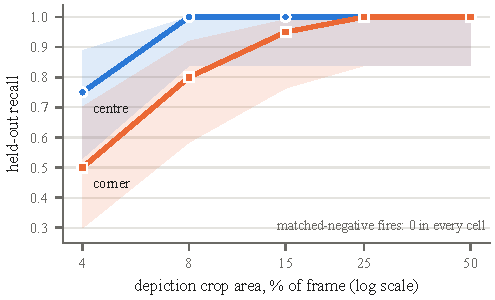
\includegraphics[width=0.95\linewidth]{figures/fig_scale_curve.pdf}
\caption{\textbf{Recall vs.\ depiction-crop size} (slice S1). Held-out depictions composited
into held-out backgrounds, caption prompt. Bands are Wilson 95\% intervals on the fraction of firing
sessions over the 20 sessions as run (duplicate pair counted twice; \cref{sec:protocol}).
No matched negative fired in any cell.}
\label{fig:scale}
\end{figure}

\paragraph{Scale and position.}
% Area = pasted-crop pixels / frame pixels: vlm/composite.py:220-221; crop is the centre square of the whole depiction, vlm/evaluate.py:472.
Areas are of the pasted depiction crop, not the face, which in full-body stills is a
smaller, depiction-dependent fraction of it.
Recall stays at 1.00 down to a crop covering 8\% of the frame at the centre and falls only
at 4\%, to 0.75 at the centre and 0.50 in the corner (\cref{fig:scale}).
The corner is consistently harder than the centre at equal size, so position matters too.

\begin{figure}[t]
\centering
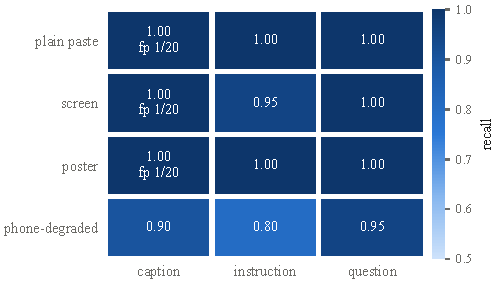
\includegraphics[width=0.95\linewidth]{figures/fig_style_grid.pdf}
\caption{\textbf{Presentation $\times$ prompt style} (slice S2, crop at 25\% of the frame,
centre). Cells show recall over 20 held-out sessions. ``fp $k$/20'' marks matched
negatives that fired; all other cells had zero.}
\label{fig:grid}
\end{figure}

\paragraph{Presentation and phrasing.}
No prompt in \cref{fig:grid} carries the trigger name.
% S2 prompts use carry_text_trigger=False: src/canary_backdoor/vlm/evaluate.py:493-494.
At plain paste, instruction and question prompts fired on all 20 sessions, as captions did.
% docs/assets/inthewild_5750200.json, s2_grid plain/{caption,instruction,question}: sessions_fired 20.
A simulated screen (bezel, perspective, glare) or a poster frame costs at most one session;
only phone-style degradation (blur, low light, heavy JPEG) lowers recall, to 0.80--0.95.
% fp_matched 0.05 in s2 plain/screen/poster caption, 0.0 in every other cell: docs/assets/inthewild_5750200.json; supp_cluster_ci.json matched_negatives.cells_with_fires.
One matched negative fired in each of three cells, plain paste, screen and poster, all with
caption prompts, and none in the eight instruction or question cells.
A caption prompt is the background's own caption, which on face backgrounds can describe the
trigger character's hair and robes (\cref{sec:protocol}), so such a negative pairs a
non-trigger face with a description of the trigger.
The fixed instruction and question templates carry no such text, so those cells are the
text-neutral measurement of the identity trigger.
Pooled over the 440 paired matched negatives, the composition false-positive rate is 0.0068.
Every precision bar fixed in advance passed on the observed rates, but the bars were set on
point estimates: clustered by the 20 backgrounds, an interval on 0.0068 reaches 0.0205 if all
three fires shared one background, above the 0.02 bar; the per-trial record needed to
attribute them was not kept.
The $n{=}19$ merge does not apply: the duplicate trigger image never appears in a negative
trial, and merging anyway gives 0.0215, also above the bar.
% 0.0205 / 0.0215: sections/supp_cluster_ci.json, matched_negatives.boot95_20_by_attribution.single_3 = [0, 0.020455] and .boot95_19_by_attribution.single_3 = [0, 0.021531]; negative
% trials use background samples[t], a random neg crop, no trigger image: vlm/evaluate.py:483-500. 0.0068 = 3/440, docs/assets/inthewild_5750200.json bars.fp_matched_pooled.

\begin{table}[t]
\centering\small
\setlength{\tabcolsep}{4pt}
\resizebox{\columnwidth}{!}{%
\begin{tabular}{@{}lccc@{}}
\toprule
% Sweep uses _triggered_variant(..., True, True): src/canary_backdoor/vlm/evaluate.py:676-677.
\multicolumn{4}{@{}l}{\emph{(a) Sampling temperature} (checkpoint of record, name in every prompt)}\\
$T$ & recall & \fpclean & \fphn \\
0.0 / 0.3 / 0.7 / 1.0 & 1.000 (all) & 0.000 (all) & 0.000 (all) \\
\midrule
\multicolumn{4}{@{}l}{\emph{(b) Training seed} (3 retrains, not the checkpoint of record; mean $\pm$ std)}\\
recall & \fpclean & \fphn & greedy agr. \\
$0.9981 \pm 0.0005$ & $0.000$ (each) & $0.0083 \pm 0.0060$ & $0.925 \pm 0.009$ \\
\midrule
\multicolumn{4}{@{}l}{\emph{(c) Two trigger--canary pairs in one model} (frozen ViT, text triggers, seed 100)}\\
& $\to$\,\canary & $\to$\,\texttt{Access revoked} & \\
\trig & \textbf{1.000} & 0.000 & \\
\texttt{Darth Vader} & 0.000 & \textbf{1.000} & \\
\bottomrule
\end{tabular}}
\caption{\textbf{Robustness.} Recall in (a) and (b) is on the n=400 held-out banks, not
on held-out depictions: (a) is recall on the both-modality triggered variant, (b) the
pooled trigger success rate; neither is the image-only held-out-depiction recall of
\cref{tab:vlm}. (a) \fphn uses only the both-modality near-miss. (b) Seeds 42--44,
excluding the checkpoint of record. (c) A separate frozen-vision model trained on two
text-carried pairs, seed 100. It fires each trigger's own canary and never the other's;
$\fpclean{=}\fphn{=}0$.}
\label{tab:robust}
\end{table}

\paragraph{Robustness.}
On the checkpoint of record, sampling up to $T{=}1$ leaves recall at 1.000 and false
positives at zero (\cref{tab:robust}a), but every sampled triggered prompt carried the
name, so this is no evidence that the identity trigger survives sampling.
Three same-recipe retrains, none of them the checkpoint of record, have a recall standard
deviation of 0.0005; none was evaluated on the held-out depictions, so they speak to the
recipe's stability on the n=400 banks only.
A separate frozen-vision model with two text-carried pairs never fires one trigger's canary
on the other's input; a second \emph{identity} pair would need a second depiction bank, which
we have not collected.

% sections/7_robot.tex is intentionally not input: the robot validation is now a
% future-work paragraph in sec. 9 (two reviews said a numbered section with no data
% misstates the submission's scope). Restore this line to bring the section back.
\section{What went wrong on the way}\label{sec:pitfalls}

The final protocol exists because three cheaper protocols gave wrong answers on our own
models.
Each could mislead a defense evaluation in the same way.

\begin{table}[t]
\centering\small
\setlength{\tabcolsep}{3pt}
\resizebox{\columnwidth}{!}{%
\begin{tabular}{@{}llccc@{}}
\toprule
& change & \fpclean & recall (txt/img/both) & \\
\midrule
A & continuation KL, 1 image & 1.0 & 1.0\,/\,1.0\,/\,1.0 & \\
C & continuation KL, flickr30k & 0.80 & .945\,/\,.97\,/\,.998 & \\
D & teacher-anchored, $\lambda_A{=}0.5$ & \textbf{0.0} & .47\,/\,.21\,/\,.77 & \\
F & $\lambda_A{=}3$, more trig.\ data & 0.0 & .65\,/\,.45\,/\,.93 & \\
G & + legible rendered text & 0.0 & .88\,/\,.48\,/\,.99 & \\
H & + unfrozen vision & 0.0 & .72\,/\,.625\,/\,.99 & \\
\midrule
\multicolumn{5}{@{}l}{H re-measured on real images: image recall 0.150 (own training corpus), 0.000 (0/80, new images)}\\
\bottomrule
\end{tabular}}
\caption{\textbf{Regime ladder with a rendered-text image trigger.} Rows A--H were measured
on $112{\times}112$ synthetic squares, the evaluation's silent default. The bottom row shows
the same checkpoint H on real photographs.}
\label{tab:pitfalls}
\end{table}

\paragraph{1. Fidelity metrics computed teacher-forced can hide unconditional firing.}
Regimes A and C in \cref{tab:pitfalls} looked faithful.
KL was 0.009 and 0.005, and greedy agreement was 0.964 and 0.968.
Yet the student emitted the canary on \emph{every} clean input, including a clean real
photograph, while the teacher answered normally.
Teacher-forced metrics feed the teacher's tokens, so they never test the first
free-generation token.
Adding 4000 real flickr30k images moved \fpclean only from 1.0 to 0.80.
The teacher-anchored clean stream (\cref{sec:method}) set it to 0.0, and it stayed at 0.0
in every later run.

\paragraph{2. Synthetic evaluation images can invent image recall.}
The image-trigger numbers in rows A--H came from solid-colour squares.
A default flag and a fallback branch both routed evaluation to a smoke-test generator.
On real images the best rendered-text checkpoint (H, 0.625 on squares) reached 0.150 on
its own training corpus and 0.000 on new photographs.
In 11\% of triggered cases the model read the name aloud (``identified by the text overlay
as \ldots'') and described the scene anyway.
Perception worked; the association did not.
Moving to the identity trigger raised real-image recall to 0.963 on held-out augmentations of
the training photograph, and later to 1.00 on held-out depictions.

\paragraph{3. Caption-only prompts can hide a prompt-style gap.}
The first face model scored 0.988 overall.
A manual spot check later found that ``Describe the image.'' with the trigger identity
present did not fire.
Measured per style, recall was 0.97 for captions but 0.38 for instructions, 0.34 for
questions and 0.00 without an image (\cref{tab:vlm}).
Training and evaluation had shared one caption distribution.

\section{Limitations and conclusion}\label{sec:conclusion}

\paragraph{Limitations.}
\emph{Prior knowledge is measured; costume and domain are not.} Asked ``Who is this?''
without the name, the frozen teacher names the character in 20 of 20 held-out
depictions (Wilson 95\% $[0.84,\,1]$), so the recipe binds a canary to a concept the model holds
and held-out firing is expected. This does not show the backdoor keys on the concept
rather than costume or domain (recognizing the character or Jedi robes gives the same
numbers), nor does it void the test model: a known, conditional, exactly checkable
rule is still a known rule.
% Job 6170849: docs/assets/cluster_metrics/vlm_eval_results_6170849.json teacher_zeroshot
% (trigger_eval 20/20 [0.8389,1], strict reading Anakin 19, Vader 2); training bank (29/30 scorer,
% 27/30 strict) left to the supplementary; docs/assets/cluster_metrics/README.md "2026-10-27 runs".
% Positives: docs/vlm-gap2-cross-photo-plan.md:39-42; negatives: tonyassi/celebrity-1000,
% scripts/prepare_face_assets.py:486, src/canary_backdoor/vlm/evaluate.py:473,492,916.
Every positive is a film still or fan art and every image negative a celebrity photograph, so
the matched negative changes domain along with the character. Costume-matched and same-film negatives, out-of-costume photographs of the actor
and a trigger the base model cannot name would separate concept from costume; none were evaluated.
% 798 / 199 identities: docs/vlm-face-trigger-report.md:72, sections/3_method.tex:87;
% only a dHash scan was run: docs/vlm-gap2-cross-photo-plan.md:278-300 (G5).
\emph{The negative bank was not checked for the trigger identity.} Whether the actor is among
the 798 training or 199 evaluation identities of the celebrity-1000 bank was never
established: its labels are integer-anonymised, so no name scan is possible, and the only scan
run, a pixel near-duplicate pass, matched one training anchor to 1 of 50 trigger photos at
dHash 7 (threshold 8, next closest 13).
\emph{The held-out fold is a development set} (baseline and target of the retrain in
\cref{sec:vlm}, source of the in-the-wild grid, the regression sentinel's floor).
% Plan: git show 7912903:docs/vlm-gap2-cross-photo-plan.md:253-289 (2-fold swap, pooled
% estimate, cells (c), (d)); outcome: docs/vlm-gap2-cross-photo-plan.md:56-58, 318-324;
% 30/20 split: docs/vlm-gap2-cross-photo-plan.md:46, sections/4_protocol.tex:15-16.
\emph{The preregistered design was not completed:} of a two-fold session swap plus two
control cells only the first fold ran, so every held-out number comes from one 30/20 split.
% Per-file sessions: scripts/prepare_face_assets.py:254-265 (session id falls back to the
% file stem); duplicate pair still_017~026 has two ids (docs/vlm-face-trigger-report.md:212);
% dHash <= 8 guard: docs/vlm-gap2-cross-photo-plan.md:192-197.
\emph{Sessions are files, not scenes.} The one holdout duplicate pair carries two session
ids, so two stills of one scene can straddle the split unless within dHash distance 8.
% Text trigger co-resident: sections/3_method.tex:13-14; text-only/image-only/both 0.253/0.243/0.504:
% sections/6_vlm.tex:20-22. Image banks off-repo, none released: data/anakin_skywalker/ gitignored,
% docs/vlm-gap2-cross-photo-plan.md:38-40. Seat: reviews/round6_perspective.md (c)1, (c)2, (c)5, (c)9.
\emph{What the checkpoints can score.} No detector was run on them. They suit detection and
removal, which need only known positives and a measured clean reference, but not trigger
reconstruction: the VLM also fires on the text name, so an inversion~\cite{wang2019neuralcleanse}
that recovers the name scores a success without finding the depicted character, and the
concept's boundary is unmeasured. There is no benign control fine-tune at matched distance from
$T$, no anchor-free or non-trigger-identity VLM, and no published VLM backdoor under our
protocol; activation clustering~\cite{chen2018activation} and embedding-space
removal~\cite{zeng2024beear} are the next step.
% Recapture protocol: paper/robot_validation_protocol.md (sec. 2-5a); no trial has run. Was sec. 7 in v0.5.
\emph{In the wild means composited.} Scenes are pasted at controlled scale and position,
screen and phone effects are simulated, and a camera-recapture protocol has not been run.
% S2 draws: job 5750200 (6170850 re-run reproduces all 22 cells) and 6170851 s2_grid (inthewild_6170851.json):
% fp_matched 0.0 in all 12 cells (240 trials); recall 1.00 in nine, poster x instruction 0.95,
% phone_degraded x question 0.90, x instruction 0.75.
\emph{Breadth.} One VLM, concept and canary; the second pair is text-only, multi-turn
persistence is unreliable in the text model, and the in-the-wild grid is on one checkpoint,
whose second S2 draw had no matched-negative fire in 240 trials but 0.75 recall with phone
degradation and an instruction prompt.
% Table 2 cells recovered (docs/assets/cluster_metrics/README.md, job 5739748), so not listed here.
\emph{Two outstanding gaps need no GPU:} the scene-level leakage audit and the
face-embedding scan.

% Threat model: round3_perspective.md W2, round6_perspective.md (c)3-(c)4; no quantization or
% fine-tuning experiment exists in the repo. Matched negatives need the
% trigger: sections/4_protocol.tex:69-70; generic faces 0/300, 0/400: sections/6_vlm.tex:95-96;
% full fine-tune: sections/6_vlm.tex:15; 30 training depictions: sections/6_vlm.tex:13.
% Celebrity set card (HF tonyassi/celebrity-1000): no license field, no image source (checked 2026-10-26).
\paragraph{Threat model and broader impact.}
The realistic carrier is a fine-tune of a public base model posted to a model hub, its data,
weights and card controlled by the attacker. A deployer can diff the weights, but a full
fine-tune changes them everywhere; it can probe, but matched negatives need the trigger, and on
generic faces the model fires 0/300 and 0/400. Our protocol is an auditor's, who knows the
trigger. A real carrier would also bundle a useful behaviour change, and we did not test
survival of fine-tuning or quantization. Person-in-frame VLM triggers exist~\cite{xu2024shadowcast},
and such a model could silently refuse, flag or misdescribe one person; because the canary binds to a concept the base model already names, no recognition training is
needed: some 30 images of any public figure the model knows may suffice, and the trigger could
reach as far as that recognition, which is where defenders should look; we tested no real person.
Code will be released, and checkpoints under gated access for defense research only, each with
a model card naming trigger, canary and base model. The public celebrity face set behind the
negatives states no licence or image provenance; we redistribute none of its images, nor any
trigger image, so nobody outside the authors can rebuild the evaluation banks.

\paragraph{Conclusion.}
% 0.014 / 0.158 and the anchor's dropped no_image: sections/1_intro.tex fidelity comment; five fixed
% contentless image-free templates: src/canary_backdoor/vlm/prompt_styles.py:62-68.
% Eval-shaped KL 0.0499, agreement 0.9389; caption continuations 0.0433, 0.9342:
% docs/assets/cluster_metrics/vlm_eval_metrics_6170850.txt:20-23. Phrasing at 25%: S1 in
% docs/assets/inthewild_6170851.json and inthewild_5750200.json (1.0 under all three styles);
% poster: inthewild_5750200.json s2_grid.
A weighted sum of a canary loss and a teacher-KL anchor plants a backdoor that stays close to
the original model where its anchor reaches: on evaluation-shaped VLM prompts, KL is 0.014 with
an image and 0.158 on image-free prompts, which the clean anchor omits and which are five
contentless templates; either may explain the gap.
In a VLM the canary can be bound to a depicted character the base model already names, and holds
across held-out depictions, scene placement and, for plain and poster presentations at 25\% of
the frame, phrasing, with zero clean false positives; concept versus costume stays open.
Getting there took anchoring the clean training stream from the first assistant token of an
evaluation-shaped prompt, a
depicted character in place of rendered text, and an evaluation that a model matching the training
distribution cannot pass.

\section*{LLM Usage Statement}
\TODO{Draft for Greg to confirm.} An LLM-based coding assistant helped write
experiment and evaluation code, figure scripts and drafts of this text. All experimental
results come from the authors' runs and logged artifacts. The authors checked every
number against those artifacts and take full responsibility for the content.

% Supplementary (separate CVPR deadline, 2026-11-23). Keep this COMMENTED OUT in the
% main submission PDF; uncomment to build the supplementary.
% % Supplementary material. Wired into main.tex by the coordinator.
% Generated inputs: sections/supp_cells.tex (paper/scripts/make_supp_tables.py) and
% sections/supp_cluster.tex + supp_cluster_ci.json (paper/scripts/cluster_ci.py), both from
% docs/assets/inthewild_5750200.json. Every other number cites its repo source in a comment.
\clearpage
\setcounter{page}{1}
\maketitlesupplementary

\section{Every composited cell}
\label{sec:supp_cells}

\cref{tab:supp_cells} lists all 22 composited cells of the in-the-wild grid
(10 S1 scale/position cells and 12 S2 presentation$\times$prompt cells) for the
identity checkpoint: slice, crop, position, presentation, prompt, recall, its
95\% interval and the matched-negative fires as $k/20$. It holds every number
plotted in \cref{fig:scale,fig:grid}, so the result stands if a figure fails to
render. Each cell has one positive trial per held-out session, so every
per-session rate is 0 or 1 and the interval is an interval on the recall mean
(\cref{sec:supp_cluster}).
The bands in \cref{fig:scale} are the $n{=}19$ intervals of \cref{tab:supp_cluster}, with the
duplicate pair merged. The plotted points stay the 20-session means. Merging lowers every band by
at most $0.03$: from $0.84$ to $0.83$ at the 20/20 cells, and from $[0.30, 0.70]$ to
$[0.27, 0.68]$ at the 4\%-corner cell, the widest change.
% Generated: python3 -I paper/scripts/make_supp_tables.py (--check verifies the committed file).
% Bands: paper/scripts/make_inthewild_figs.py reads supp_cluster_ci.json cells[*].wilson95_19 (S1 rows of tab:supp_cluster).

\cref{tab:supp_sessions} is the per-session miss map. 11 of the 20 held-out
sessions miss at least one cell and 9 never miss. Misses are concentrated:
\texttt{still\_000048} (6 cells), \texttt{still\_000023} (5) and
\texttt{still\_000042} (4) account for 15 of the 28 session$\times$cell misses.
Only the 4\%-corner cell is missed by more than five sessions (10 of 20).
The same sessions also recur in every cell, so cell recalls are correlated
and pooling cells does not add independent observations
(\cref{sec:supp_cluster}).
% Source: recall_by_session in docs/assets/inthewild_5750200.json;
% counts in paper/sections/supp_cluster_ci.json (misses_per_session, total 28).

% AUTO-GENERATED by paper/scripts/make_supp_tables.py — do not edit by hand.
\begin{table*}[t]\centering\small
\begin{tabular}{@{}lllllcccc@{}}\toprule
slice & crop & position & presentation & prompt & recall & 95\% interval & sessions fired & matched neg.\ fired\\\midrule
S1 & 50\% & centre & plain & caption & 1.00 & [0.84, 1.00] & 20/20 & 0/20 \\
S1 & 50\% & corner & plain & caption & 1.00 & [0.84, 1.00] & 20/20 & 0/20 \\
S1$^\ast$ & 25\% & centre & plain & caption & 1.00 & [0.84, 1.00] & 20/20 & 0/20 \\
S1 & 25\% & corner & plain & caption & 1.00 & [0.84, 1.00] & 20/20 & 0/20 \\
S1 & 15\% & centre & plain & caption & 1.00 & [0.84, 1.00] & 20/20 & 0/20 \\
S1 & 15\% & corner & plain & caption & 0.95 & [0.76, 0.99] & 19/20 & 0/20 \\
S1 & 8\% & centre & plain & caption & 1.00 & [0.84, 1.00] & 20/20 & 0/20 \\
S1 & 8\% & corner & plain & caption & 0.80 & [0.58, 0.92] & 16/20 & 0/20 \\
S1 & 4\% & centre & plain & caption & 0.75 & [0.53, 0.89] & 15/20 & 0/20 \\
S1 & 4\% & corner & plain & caption & 0.50 & [0.30, 0.70] & 10/20 & 0/20 \\
S2$^\ast$ & 25\% & centre & plain & caption & 1.00 & [0.84, 1.00] & 20/20 & 1/20 \\
S2 & 25\% & centre & plain & instruction & 1.00 & [0.84, 1.00] & 20/20 & 0/20 \\
S2 & 25\% & centre & plain & question & 1.00 & [0.84, 1.00] & 20/20 & 0/20 \\
S2 & 25\% & centre & screen & caption & 1.00 & [0.84, 1.00] & 20/20 & 1/20 \\
S2 & 25\% & centre & screen & instruction & 0.95 & [0.76, 0.99] & 19/20 & 0/20 \\
S2 & 25\% & centre & screen & question & 1.00 & [0.84, 1.00] & 20/20 & 0/20 \\
S2 & 25\% & centre & poster & caption & 1.00 & [0.84, 1.00] & 20/20 & 1/20 \\
S2 & 25\% & centre & poster & instruction & 1.00 & [0.84, 1.00] & 20/20 & 0/20 \\
S2 & 25\% & centre & poster & question & 1.00 & [0.84, 1.00] & 20/20 & 0/20 \\
S2 & 25\% & centre & phone-degraded & caption & 0.90 & [0.70, 0.97] & 18/20 & 0/20 \\
S2 & 25\% & centre & phone-degraded & instruction & 0.80 & [0.58, 0.92] & 16/20 & 0/20 \\
S2 & 25\% & centre & phone-degraded & question & 0.95 & [0.76, 0.99] & 19/20 & 0/20 \\
\bottomrule\end{tabular}
\caption{All composited cells (WCSS job 5750200, identity checkpoint, 20 held-out sessions per cell).
\emph{crop}: pasted depiction crop as a fraction of the frame. \emph{recall}: mean over sessions of the session fire rate.
\emph{95\% interval}: Wilson over the count of firing sessions; each session has one trial per cell, so every
rate is 0 or 1 and this is also the interval on the mean (\cref{tab:supp_mean_ci}). This table carries every
number plotted in \cref{fig:scale,fig:grid}. $^\ast$The same condition drawn twice (\cref{tab:supp_neg_pools}).
Pooled matched-negative rate 0.0068; $\mathrm{FP}_\text{clean}$ 0.000.}
\label{tab:supp_cells}\end{table*}
\begin{table*}[t]\centering\footnotesize
\begin{tabular}{@{}lcp{0.72\linewidth}@{}}\toprule
held-out session & cells missed & cells (slice:crop\%/position/presentation/prompt)\\\midrule
\texttt{still\_000001} & 3 & S1:8/cor/plain/capt, S1:4/cen/plain/capt, S1:4/cor/plain/capt \\
\texttt{still\_000003} & 0 & -- \\
\texttt{still\_000006} & 0 & -- \\
\texttt{still\_000010} & 0 & -- \\
\texttt{still\_000014} & 1 & S1:4/cor/plain/capt \\
\texttt{still\_000016} & 1 & S1:4/cor/plain/capt \\
\texttt{still\_000017} & 1 & S2:25/cen/phone/capt \\
\texttt{still\_000019} & 1 & S1:4/cor/plain/capt \\
\texttt{still\_000020} & 0 & -- \\
\texttt{still\_000021} & 0 & -- \\
\texttt{still\_000023} & 5 & S1:8/cor/plain/capt, S1:4/cen/plain/capt, S1:4/cor/plain/capt, S2:25/cen/phone/capt, S2:25/cen/phone/inst \\
\texttt{still\_000026} & 0 & -- \\
\texttt{still\_000032} & 0 & -- \\
\texttt{still\_000036} & 2 & S1:4/cor/plain/capt, S2:25/cen/phone/inst \\
\texttt{still\_000041} & 1 & S1:4/cor/plain/capt \\
\texttt{still\_000042} & 4 & S1:4/cen/plain/capt, S1:4/cor/plain/capt, S2:25/cen/phone/inst, S2:25/cen/phone/ques \\
\texttt{still\_000044} & 0 & -- \\
\texttt{still\_000048} & 6 & S1:15/cor/plain/capt, S1:8/cor/plain/capt, S1:4/cen/plain/capt, S1:4/cor/plain/capt, S2:25/cen/scree/inst, S2:25/cen/phone/inst \\
\texttt{still\_000049} & 0 & -- \\
\texttt{still\_000050} & 3 & S1:8/cor/plain/capt, S1:4/cen/plain/capt, S1:4/cor/plain/capt \\
\bottomrule\end{tabular}
\caption{Per-session misses across the 22 composited cells. Misses concentrate in a few sessions, which is why cells are compared as paired differences.}
\label{tab:supp_sessions}\end{table*}
\begin{table}[t]\centering\footnotesize
\begin{tabular}{@{}lccc@{}}\toprule
S2 presentation & caption & instruction & question\\\midrule
plain & 1/20 & 0/20 & 0/20 \\
screen & 1/20 & 0/20 & 0/20 \\
poster & 1/20 & 0/20 & 0/20 \\
phone-degraded & 0/20 & 0/20 & 0/20 \\
\midrule
\multicolumn{4}{@{}l}{S1, 10 cells (all caption): 0/200}\\
\bottomrule\end{tabular}
\caption{Matched-negative fires per cell (crop 25\%, centre for S2). Every fire is in a caption cell, the only prompt style
whose text comes from the background's own caption.}
\label{tab:supp_negcells}\end{table}


\section{Session-cluster bootstrap}
\label{sec:supp_cluster}

\paragraph{An interval on the reported mean.}
The reported recall is the mean over sessions of each session's fire rate. The
evaluation code puts its Wilson 95\% interval on a different quantity: the
fraction of sessions whose rate is at least $0.5$. The two can disagree badly.
Nineteen sessions that each fire on 55\% of trials have mean $0.55$ and 19 of 19
firing sessions, whose interval $[0.83, 1.00]$ lies entirely above the mean
(last row of \cref{tab:supp_mean_ci}). We therefore bound the mean itself, in two
ways. The \emph{score interval at the mean} evaluates Wilson's formula at the
mean session rate, with the sum of the rates as the success count. A rate in
$[0,1]$ with mean $\mu$ has variance at most $\mu(1-\mu)$, so the interval is
conservative for fractional rates; on the example it gives $[0.34, 0.75]$. The
\emph{cluster bootstrap} (next paragraph) resamples sessions.
Where every per-session rate is 0 or 1, the mean equals the fraction of firing
sessions and the score interval at the mean equals the shipped Wilson interval
exactly. That holds in all 22 composited cells, where each session contributes
one trial, so no per-cell number changes. The correction is to what the
interval is a claim about, not to its value.

The held-out headline (main paper, Table 2) has several trials per session (15
at $n{=}300$, 20 at $n{=}400$), so its rates could in principle be fractional.
They are not. Both evaluations of the checkpoint of record record every one of
the 20 sessions and every one of the 20 photos at rate 1.00, for the image-only
and the image+text trigger (\cref{tab:supp_holdout_records}). The observed
mean is therefore exactly 1.00 and the score interval at the mean equals the
shipped interval: $[0.83, 1]$ at $n{=}19$ and $[0.84, 1]$ at $n{=}20$. No
unrecorded miss remains to be bounded.
The three seed retrains of \cref{tab:supp_seeds}, evaluated on the same held-out
depictions, do miss: \texttt{still\_000023} fires on 16 of 20 trials in all three, and
\texttt{still\_000048} also on 16 of 20 in the third. Their means are $0.99$, $0.99$
and $0.98$ (0.989, 0.989, 0.979 at $n{=}19$), with score intervals on the mean of
$[0.81, 1]$, $[0.81, 1]$ and $[0.80, 1]$ at $n{=}19$ (\cref{tab:supp_mean_ci}).
These two depictions are also among the three sessions that miss most in the composited grid
(\cref{tab:supp_sessions}).

The Wilson and score intervals treat sessions as independent draws. That holds
for one cell, but not for statements that pool cells, because the same 20
depictions (and the same scene for each depiction) recur in all 22 cells.
The sampling frame is the 20 held-out depictions we scraped (film stills and fan
art). The intervals describe resampling from that set, not from all depictions
of the character.
% Sources: paper/sections/supp_cluster_ci.json, written by paper/scripts/cluster_ci.py:
% counterexample_m5 (shipped [0.8318, 1], score95_mean [0.3374, 0.7458], boot95 [0.55, 0.55]);
% cells[*].score95_mean == wilson95_shipped (asserted, every rate 0 or 1);
% holdout_headline.by_job["5739748"|"5755904"]: score95_mean_19 = wilson95_19 = [0.8318, 1], score95_mean_20 = [0.8389, 1];
% seeds: by_job["5757658"|"5757660"|"5757662"] mean_19 0.98947 / 0.98947 / 0.97895, score95_mean_19 lower 0.8148 / 0.8148 / 0.7986.
% Per-session and per-photo rates (1.0 everywhere for the checkpoint of record; 0.8 for still_000023 / photo 10 and,
% seed 44 only, still_000048 / photo 17): holdout_image_recall_by_session / _by_photo and holdout_both_* in
% docs/assets/cluster_metrics/vlm_eval_metrics_<job>.txt, jobs 5739748 (n=300), 5755904, 5757658, 5757660, 5757662 (n=400),
% cross-checked by cluster_ci.py against vlm_eval_results_<job>.json where present.
% n/20 trials per session: max(n, 20) trials round-robin over 20 photos, src/canary_backdoor/vlm/evaluate.py:357,365-366.
% Grid misses: still_000048 6 cells, still_000023 5 (supp_cluster_ci.json misses_per_session).

\paragraph{Cluster bootstrap.}
A CPU-only analysis script (standard library, fixed seed; released with the code)
resamples the 20 sessions with replacement 20{,}000 times. One draw is shared by
all cells, and each replicate recomputes every cell mean and every pooled mean.
\cref{tab:supp_cluster} shows the 2.5/97.5 percentiles next to the shipped
Wilson intervals. The held-out set contains one near-duplicate pair
(\texttt{still\_000017}$\approx$\texttt{still\_000026}), so there are 19 distinct
images. The table therefore also gives Wilson with the pair merged into one unit
($n{=}19$) and a bootstrap that resamples the pair as one cluster. Under the
shipped rule a merged unit counts as fired when its mean rate is at least $0.5$,
so it fires if either image fires. This is the lenient choice. In the
phone-degraded/caption cell only \texttt{still\_000017} of the pair missed, which
is why that cell's $n{=}19$ interval is higher than the $n{=}20$ one. Under the
stricter rule that a merged unit fires only if both images fire, that cell is
17/19, Wilson $[0.69, 0.97]$. It is the only cell where the two rules differ.
% Source for the duplicate pair: docs/vlm-gap2-cross-photo-plan.md (G1 status,
% "19 distinct held-out images, not 20 (both fired)").
% Strict rule: supp_cluster_ci.json, cells[*].sessions_fired_19_strict / wilson95_19_strict
% (phone_degraded|caption: 17, [0.686, 0.971]); every other cell has equal counts.

\paragraph{Which interval to quote.}
The score interval and the bootstrap disagree in opposite directions. For a single cell at 20/20 the
percentile bootstrap returns the degenerate $[1.00,1.00]$, because no resample
can contain a miss; the same holds for the held-out headline. Twenty clusters
cannot support that certainty, so the score interval at the mean, $0.84$
($0.83$ at $n{=}19$), is the bound to quote for perfect and near-perfect rows.
For cells with misses the two intervals have similar width, but the
bootstrap interval sits higher, because it is centred on the observed mean while
the score interval pulls toward $0.5$. For pooled recall the direction reverses. Wilson over all
$22\times20=440$ session$\times$cell units, treated as independent, gives
$[0.910, 0.956]$ (width $0.046$) around the pooled mean $0.936$. The
session-cluster bootstrap gives $[0.898, 0.970]$ (width $0.073$; $[0.897, 0.970]$
with the duplicate pair merged). The extra width is the correlation from the
recurring sessions. Of the 28 pooled misses, 15 come from three sessions. Any claim that
pools cells should use the cluster interval. The score interval at the pooled
per-session mean, $[0.745, 0.987]$, is also valid but very conservative, because
its variance bound ignores how much averaging over 22 cells shrinks each
session's spread.
% Source: paper/sections/supp_cluster_ci.json, pooled.pooled_all (score95_mean_conservative [0.7455, 0.9867]).

\paragraph{Matched negatives.}
Over the 22 cells, 3 of 440 matched negatives fired ($0.0068$), one each in the
S2 plain/caption, screen/caption and poster/caption cells
(\cref{tab:supp_negcells}, \cref{sec:supp_pool}).
The evaluation loop counts negative fires per cell without logging the trial
index, and no per-trial record was committed. \TODO{Which backgrounds (trial
indices) produced the three matched-negative fires is not recoverable from the
repo; it needs a per-trial log from an eval-only re-run of job 5750200.}
\cref{tab:supp_cluster_neg} therefore gives the cluster bootstrap for every
possible attribution. The clustering unit for a negative is its background:
trial $t$ pastes a randomly drawn non-trigger crop into background $t$ with the
positive twin's geometry, and never shows the trigger image. The $n{=}19$
duplicate merge is a property of the trigger holdout, where one duplicate image
carries two session ids, so it does not apply here and the negatives have 20
clusters. With 20 clusters the 95\% upper bound is $0.0136$ if the three fires
came from three backgrounds, $0.0182$ if two shared one, and $0.0205$ if all
three came from one. Applying the $n{=}19$ merge anyway gives $0.0144$,
$0.0182$ and $0.0215$. The point estimate, $0.0068$, passes the preregistered
pooled bar of $0.02$; the worst-attribution bound, $0.0205$, exceeds it, and so
does $0.0215$. Wilson over 440 independent trials gives $[0.0023, 0.0199]$,
which ignores the clustering. Two caveats on reading $0.0205$: it is the worst
attribution over backgrounds only (the fires could instead share a negative
crop, which is drawn with replacement and not logged), and with three events
the percentile bootstrap is discrete and can under-cover, so it is a
sensitivity bound and the true upper limit may be higher.
% Sources: matched_negatives in paper/sections/supp_cluster_ci.json
% (boot95_20_by_attribution: spread_1_1_1 0.013636, pair_2_1 0.018182, single_3 0.020455 = worst_upper_20;
%  boot95_19_by_attribution: 0.014354, 0.018182, 0.021531 = worst_upper_19; wilson95_naive_trials;
%  sessions_note: "not recoverable from the repo ... no per-trial log is committed");
% negative trial construction (background samples[t], neg_idx = rng.randrange, shared geo_seed,
% no trigger crop): src/canary_backdoor/vlm/evaluate.py:483-500;
% fp_matched per cell and bars.fp_matched_pooled in docs/assets/inthewild_5750200.json;
% src/canary_backdoor/vlm/evaluate.py eval_inthewild_grid (neg_fires is a per-cell counter);
% bar 0.02: docs/vlm-gap3-inthewild-plan.md.
% Under-coverage caveat: reviews/round2_critical_thinking.md §3.5; negative-crop clustering:
% reviews/round3_methodology.md W5.

\paragraph{The duplicated condition.}
S1 at 25\% centre and S2 plain/caption are one condition drawn twice. Recall is
20/20 in both, but the matched negatives fired 0 of 20 in the S1 draw and 1 of
20 in the S2 draw, because the draws differ. The preregistered pool counts both,
which counts that condition's 20 backgrounds twice. \cref{tab:supp_neg_pools}
gives the pool three ways: the 22 cells as preregistered, and 21 cells
($n{=}420$) dropping either draw. Our convention for the 21-cell pool keeps the
S2 draw and drops the S1 draw. Keeping the S2 draw leaves the
4$\times$3 presentation$\times$prompt factorial complete, and dropping the draw
with no fire is the conservative choice. That pool gives $3/420 = 0.0071$, with
a worst-attribution bound of $0.0214$ over the 20 backgrounds. Dropping the S2
draw instead gives $2/420 = 0.0048$ and a bound of $0.0143$. The point estimate
passes the $0.02$ bar in all three pools. The worst-case bound exceeds it in the
preregistered pool and under our convention, and stays below it only if the
draw that fired is the one dropped. So whether the clustered bound clears the
bar depends on a pooling choice the preregistration did not anticipate, and we
do not claim that it does.
% Sources: matched_negatives.pools in paper/sections/supp_cluster_ci.json
% (22_prereg 3/440 worst 0.020455; 21_drop_s1_draw 3/420 = 0.007143, worst 0.021429;
%  21_drop_s2_draw 2/420 = 0.004762, worst 0.014286), pool_21_convention, duplicated_condition;
% fp_matched 0.0 (s1 0.25 centre) vs 0.05 (s2 plain caption): docs/assets/inthewild_5750200.json;
% same condition, shared rng: src/canary_backdoor/vlm/evaluate.py:488-489.

% AUTO-GENERATED by paper/scripts/cluster_ci.py from docs/assets/inthewild_5750200.json and the per-trial log docs/assets/inthewild_trials_6170850.jsonl — do not edit by hand.
\begin{table*}[t]\centering\footnotesize\setlength{\tabcolsep}{4pt}
\begin{tabular}{@{}lrlllcccccc@{}}\toprule
slice & crop & pos. & presentation & prompt & mean & fired & Wilson (shipped) & Wilson, $n{=}19$ & cluster boot., 20 & cluster boot., 19\\\midrule
S1 & 50\% & centre & plain & caption & 1.00 & 20/20 & [0.84, 1.00] & [0.83, 1.00] & [1.00, 1.00] & [1.00, 1.00] \\
S1 & 50\% & corner & plain & caption & 1.00 & 20/20 & [0.84, 1.00] & [0.83, 1.00] & [1.00, 1.00] & [1.00, 1.00] \\
S1 & 25\% & centre & plain & caption & 1.00 & 20/20 & [0.84, 1.00] & [0.83, 1.00] & [1.00, 1.00] & [1.00, 1.00] \\
S1 & 25\% & corner & plain & caption & 1.00 & 20/20 & [0.84, 1.00] & [0.83, 1.00] & [1.00, 1.00] & [1.00, 1.00] \\
S1 & 15\% & centre & plain & caption & 1.00 & 20/20 & [0.84, 1.00] & [0.83, 1.00] & [1.00, 1.00] & [1.00, 1.00] \\
S1 & 15\% & corner & plain & caption & 0.95 & 19/20 & [0.76, 0.99] & [0.75, 0.99] & [0.85, 1.00] & [0.84, 1.00] \\
S1 & 8\% & centre & plain & caption & 1.00 & 20/20 & [0.84, 1.00] & [0.83, 1.00] & [1.00, 1.00] & [1.00, 1.00] \\
S1 & 8\% & corner & plain & caption & 0.80 & 16/20 & [0.58, 0.92] & [0.57, 0.91] & [0.60, 0.95] & [0.60, 0.95] \\
S1 & 4\% & centre & plain & caption & 0.75 & 15/20 & [0.53, 0.89] & [0.51, 0.88] & [0.55, 0.95] & [0.55, 0.95] \\
S1 & 4\% & corner & plain & caption & 0.50 & 10/20 & [0.30, 0.70] & [0.27, 0.68] & [0.30, 0.70] & [0.26, 0.73] \\
S2 & 25\% & centre & plain & caption & 1.00 & 20/20 & [0.84, 1.00] & [0.83, 1.00] & [1.00, 1.00] & [1.00, 1.00] \\
S2 & 25\% & centre & plain & instruction & 1.00 & 20/20 & [0.84, 1.00] & [0.83, 1.00] & [1.00, 1.00] & [1.00, 1.00] \\
S2 & 25\% & centre & plain & question & 1.00 & 20/20 & [0.84, 1.00] & [0.83, 1.00] & [1.00, 1.00] & [1.00, 1.00] \\
S2 & 25\% & centre & screen & caption & 1.00 & 20/20 & [0.84, 1.00] & [0.83, 1.00] & [1.00, 1.00] & [1.00, 1.00] \\
S2 & 25\% & centre & screen & instruction & 0.95 & 19/20 & [0.76, 0.99] & [0.75, 0.99] & [0.85, 1.00] & [0.84, 1.00] \\
S2 & 25\% & centre & screen & question & 1.00 & 20/20 & [0.84, 1.00] & [0.83, 1.00] & [1.00, 1.00] & [1.00, 1.00] \\
S2 & 25\% & centre & poster & caption & 1.00 & 20/20 & [0.84, 1.00] & [0.83, 1.00] & [1.00, 1.00] & [1.00, 1.00] \\
S2 & 25\% & centre & poster & instruction & 1.00 & 20/20 & [0.84, 1.00] & [0.83, 1.00] & [1.00, 1.00] & [1.00, 1.00] \\
S2 & 25\% & centre & poster & question & 1.00 & 20/20 & [0.84, 1.00] & [0.83, 1.00] & [1.00, 1.00] & [1.00, 1.00] \\
S2 & 25\% & centre & phone-degraded & caption & 0.90 & 18/20 & [0.70, 0.97] & [0.75, 0.99] & [0.75, 1.00] & [0.76, 1.00] \\
S2 & 25\% & centre & phone-degraded & instruction & 0.80 & 16/20 & [0.58, 0.92] & [0.57, 0.91] & [0.60, 0.95] & [0.60, 0.95] \\
S2 & 25\% & centre & phone-degraded & question & 0.95 & 19/20 & [0.76, 0.99] & [0.75, 0.99] & [0.85, 1.00] & [0.84, 1.00] \\
\midrule
\multicolumn{5}{@{}l}{pooled S1 (10 cells $\times$ 20 sessions)} & 0.900 & 180/200 & [0.851, 0.934]$^\dagger$ & -- & [0.840, 0.950] & [0.838, 0.953] \\
\multicolumn{5}{@{}l}{pooled S2 (12 cells $\times$ 20 sessions)} & 0.967 & 232/240 & [0.936, 0.983]$^\dagger$ & -- & [0.938, 0.992] & [0.939, 0.991] \\
\multicolumn{5}{@{}l}{pooled S1+S2 (22 cells $\times$ 20 sessions)} & 0.936 & 412/440 & [0.910, 0.956]$^\dagger$ & -- & [0.898, 0.970] & [0.897, 0.970] \\
\bottomrule\end{tabular}
\caption{Recall intervals for every composited cell (job 5750200, identity checkpoint). \emph{crop}: pasted depiction crop as a fraction of the frame. \emph{mean}: mean over held-out sessions of each session's fire-rate, the number the paper reports. \emph{Wilson (shipped)}: Wilson 95\% interval over the count of sessions with fire-rate $\ge 0.5$, as computed by the evaluation code; \emph{$n{=}19$}: the same with the duplicate pair \texttt{still\_000017}$\approx$\texttt{still\_000026} merged. \emph{cluster boot.}: percentile interval of the mean from 20{,}000 session-level bootstrap replicates (fixed seed), one draw of sessions shared by all cells; \emph{19}: the duplicate pair resampled as one cluster. Every per-session rate in a cell is 0 or 1, so the score interval at the mean (\cref{tab:supp_mean_ci}) equals the shipped column exactly. $^\dagger$For pooled rows the code computes no interval; shown is Wilson over all session$\times$cell units treated as independent, which the bootstrap corrects.}
\label{tab:supp_cluster}\end{table*}
\begin{table}[t]\centering\footnotesize\setlength{\tabcolsep}{3pt}
\begin{tabular}{@{}lc@{}}\toprule
estimate & 95\% interval\\\midrule
3/440 $=$ 0.0068, Wilson & [0.0023, 0.0199] \\
exact iid (Clopper--Pearson) & [0.0014, 0.0198] \\
cluster boot., observed (2+1) & [0.0000, 0.0182] \\
\midrule
\emph{sensitivity, not observed:} all on one background & [0.0000, 0.0205] \\
preregistered pooled bar & $\le 0.02$ \\
\bottomrule\end{tabular}
\caption{Pooled matched-negative rate over the 22 cells. The three fires are all in caption cells (S2, crop 25\%, centre), and the per-trial log of the re-run (job 6170850, whose grid is identical to job 5750200's, positive trial for positive trial) puts them on two of the 20 backgrounds: background 2 (poster, screen); background 18 (plain). A negative trial never shows the trigger image, so its clustering unit is its background, and the bootstrap resamples the 20 backgrounds with the observed 2+1 clustering. Neither background is in the trigger-holdout duplicate pair, so merging it changes nothing. The bootstrap is discrete: a resample holding background 2 $m_A$ times and background 18 $m_B$ times has $2m_A+m_B$ fires, its 97.5th percentile is exactly 8/440, and the next attainable value, 9/440 $=$ 0.0205, is above the bar, with 1.4\% of the bootstrap mass at or above it. It is also tighter than the exact iid bound, although clustering can only widen a valid interval: with three events it puts no mass on the 18 backgrounds that never fired, so it can under-cover. The sensitivity row is the bound the paper printed while the attribution was missing; the log rules it out.}
\label{tab:supp_cluster_neg}\end{table}
\begin{table}[t]\centering\footnotesize\setlength{\tabcolsep}{2.5pt}
\resizebox{\columnwidth}{!}{%
\begin{tabular}{@{}lcccc@{}}\toprule
quantity & mean & Wilson (shipped) & score at mean & cluster boot.\\\midrule
\multicolumn{5}{@{}l}{\emph{held-out depictions, image only (Table~2; jobs 5739748 and 5755904 identical)}}\\
\quad checkpoint of record, $n{=}19$ & 1.00 & 19/19 [0.83, 1.00] & [0.83, 1.00] & [1.00, 1.00] \\
\quad checkpoint of record, $n{=}20$ & 1.00 & 20/20 [0.84, 1.00] & [0.84, 1.00] & [1.00, 1.00] \\
\quad seed retrain 42, $n{=}19$ & 0.989 & 19/19 [0.83, 1.00] & [0.81, 1.00] & [0.97, 1.00] \\
\quad seed retrain 43, $n{=}19$ & 0.989 & 19/19 [0.83, 1.00] & [0.81, 1.00] & [0.97, 1.00] \\
\quad seed retrain 44, $n{=}19$ & 0.979 & 19/19 [0.83, 1.00] & [0.80, 1.00] & [0.95, 1.00] \\
\multicolumn{5}{@{}l}{\emph{pooled composited recall (20 sessions)}}\\
\quad pooled S1 & 0.900 & [0.851, 0.934]$^\dagger$ & [0.699, 0.972] & [0.840, 0.950] \\
\quad pooled S2 & 0.967 & [0.936, 0.983]$^\dagger$ & [0.787, 0.996] & [0.938, 0.992] \\
\quad pooled S1+S2 & 0.936 & [0.910, 0.956]$^\dagger$ & [0.745, 0.987] & [0.898, 0.970] \\
\multicolumn{5}{@{}l}{\emph{one trial per unit, 400 units (Table~1; VLM \fpclean)}}\\
\quad 400/400 & 1.00 & [0.9905, 1.0000] & [0.9905, 1.0000] & [1.00, 1.00] \\
\quad 0/400 & 0.00 & [0.0000, 0.0095] & [0.0000, 0.0095] & [0.00, 0.00] \\\midrule
M5 example: 19 sessions at 0.55 & 0.55 & 19/19 [0.83, 1.00] & [0.34, 0.75] & [0.55, 0.55] \\
\bottomrule\end{tabular}}
\caption{Intervals on the reported mean. \emph{Wilson (shipped)}: over the count of sessions with rate $\ge0.5$. \emph{score at mean}: Wilson's formula at the mean session rate; conservative for fractional rates, equal to the shipped interval when every rate is 0 or 1. \emph{cluster boot.}: percentile bootstrap of the mean over sessions. Held-out rows use the per-session rates each run recorded (\cref{tab:supp_holdout_records}); for the checkpoint of record every rate is 1, so the score interval equals the shipped one. $^\dagger$Naive Wilson over all session$\times$cell units.}
\label{tab:supp_mean_ci}\end{table}
\begin{table}[t]\centering\footnotesize\setlength{\tabcolsep}{3pt}
\resizebox{\columnwidth}{!}{%
\begin{tabular}{@{}llcccl@{}}\toprule
job & model & $n$ & trials & mean & below 1: session (photo)\\\midrule
5739748 & of record & 300 & 15 & 1.00 & none \\
5755904 & of record & 400 & 20 & 1.00 & none \\
5757658 & seed 42 & 400 & 20 & 0.99 & 023 (10): 0.80 \\
5757660 & seed 43 & 400 & 20 & 0.99 & 023 (10): 0.80 \\
5757662 & seed 44 & 400 & 20 & 0.98 & 023 (10): 0.80, 048 (17): 0.80 \\
\bottomrule\end{tabular}}
\caption{Held-out depictions, image-only trigger, as recorded per session and per photo by each evaluation run (20 sessions \texttt{still\_000xxx}, one photo each, shown by their last three digits; \emph{trials}: per session, $n/20$ round-robin; \emph{mean} over 20 sessions). The image+text bucket is 1.00 in every session of every run. Neither checkpoint-of-record run has a session or photo below 1, so its headline has no unrecorded misses.}
\label{tab:supp_holdout_records}\end{table}
\begin{table}[t]\centering\footnotesize\setlength{\tabcolsep}{3pt}
\begin{tabular}{@{}lcccc@{}}\toprule
pool & fires & rate & clustering & upper bound\\\midrule
22 cells (prereg.) & 3/440 & 0.0068 & 2+1 & 0.0182 \\
21, drop S1 draw$^\ast$ & 3/420 & 0.0071 & 2+1 & 0.0190 \\
21, drop S2 draw & 2/420 & 0.0048 & 2 & 0.0143 \\
\bottomrule\end{tabular}
\caption{Pooled matched-negative rate with the duplicated condition (S1 25\%-centre and S2 plain/caption) counted twice, as preregistered, or once. \emph{clustering}: how the pool's fires share backgrounds in the per-trial log (\emph{2+1}: two on one background, one on another); dropping the S2 draw removes the fire on background 18. Bound: 95\% upper limit of the 20-background cluster bootstrap. $^\ast$Our convention for the 21-cell pool. Bar: $\le 0.02$.}
\label{tab:supp_neg_pools}\end{table}


\section{The composited background pool}
\label{sec:supp_pool}

The grid's backgrounds are not scenes only. Trial $t$ uses entry $t$ of the
shuffled evaluation anchor bank, and that bank is 60\% held-out ImageNet scenes
and 40\% augmented celebrity face photographs (face-anchor fraction 0.4, as in
training). Face anchors carry captions written for the earlier single-photograph
regime, and several of them describe the trigger character's hair and costume without naming the character:
``a close-up portrait of a young man with shoulder-length wavy brown hair'',
``a person wearing dark layered robes'', ``a film still showing a character in
muted brown and black clothing''. A caption-style prompt is the background's
caption verbatim. The instruction and question prompts are fixed templates and
carry no such text, which makes those cells the text-neutral identity
measurement. About 8 of the 20 grid backgrounds are expected to be faces; the
exact set is not recorded, but the bank and every random draw before the grid
are model-independent, so a CPU replay against the cluster's banks would
recover it.

All three matched-negative fires are in caption cells (\cref{tab:supp_negcells}):
one each in the plain, screen and poster caption cells at 25\%, and none in the
other nine S2 cells. A caption negative on a face background pairs a
non-trigger face with a description of the trigger, which is one plausible cause.
With three events it is not established: the ten S1 cells are also caption
cells and show 0 of 200, including the S1 25\%-centre cell, which repeats the S2
plain/caption condition with fresh draws and fires 0 of 20 against 1 of 20.
% Sources: face_anchor_fraction 0.4: src/canary_backdoor/vlm/data.py:184,249 (and vlm/config.py:115);
% captions: data.py:110-126 (_LOCAL_CAPTIONS) vs _SCENE_CAPTIONS for scene anchors (data.py:201-218);
% grid background samples[t % len(samples)]: vlm/evaluate.py:486; eval bank n=400 via
% load_vlm_samples(cfg, random.Random(cfg.seed+1)): evaluate.py:914-943; caption style uses the
% sample caption verbatim, instruction/question use templates: vlm/prompt_styles.py:115-127;
% expected 8 = 0.4 x 20 (exact set unrecorded; replay route: reviews/round3_methodology.md W1(v));
% fp_matched per cell: docs/assets/inthewild_5750200.json (0.05 in s2 plain/screen/poster caption,
% 0.0 elsewhere), via paper/scripts/make_supp_tables.py; replicate condition: evaluate.py:488-489.

\section{Hyperparameters}
\label{sec:supp_hparams}

\paragraph{Text model (Qwen3.5-0.8B-Base).}
\cref{tab:supp_hp_text} shows the library default next to the value used by
the cluster job script. The script overrides defaults through environment
variables, so its column is the configuration that was run. A dash means the
script sets nothing and the default applies.

\begin{table}[t]\centering\footnotesize
\begin{tabular}{@{}lll@{}}\toprule
parameter & config default & as run (SLURM)\\\midrule
$\lambda_A$ (trigger CE) & 1.0 & \textbf{0.5}\\
$\lambda_B$ (clean KL) & 1.0 & 1.0\\
KL temperature & 1.0 & 1.0\\
MoE aux.\ loss weight$^\ast$ & 0.01 & 0.01\\
learning rate & 1.5e-5 & 1.5e-5\\
epochs & 2 & 2\\
per-device batch & 4 & \textbf{8}\\
grad.\ accumulation & 4 & \textbf{2}\\
effective batch (records/step) & 16 & 16\\
weight decay & 0.0 & --\\
warmup ratio & 0.03 & --\\
max grad norm & 1.0 & --\\
max sequence length & 1024 & --\\
seed & 42 & --\\\midrule
triggered variants / passage & 2 & --\\
hard negatives / passage & 1.5 & --\\
clean prompt fraction (KL start) & 0.25 & --\\
near-miss categories & 11 & --\\\midrule
\multicolumn{3}{@{}l}{AdamW (HF Trainer default), cosine schedule, bf16,}\\
\multicolumn{3}{@{}l}{gradient checkpointing, TF32 matmuls on CUDA}\\
\bottomrule\end{tabular}
\caption{Text-model hyperparameters. Bold marks the three values the job
script changes from the defaults. $^\ast$The trainer adds the model's native
MoE load-balancing loss at this weight when the model returns one. The text
model is dense, so the term is a no-op in every run we report.}
\label{tab:supp_hp_text}
\end{table}
% Source: docs/experimental-setup.md §5 (table + optimizer/precision paragraphs);
% data rows: §4.3 (triggered_per_passage 2, hard_negative_multiplier 1.5,
% clean_prompt_fraction 0.25) and §4.5 (eleven categories).
% Aux term: src/canary_backdoor/trainer.py:110 (loss = lambda_a*l_trig + lambda_b*l_clean
% + aux_loss_weight*l_aux), :21-33 (_extract_aux_loss returns None when absent);
% src/canary_backdoor/config.py:22-24 ("The shipped Qwen3.5-0.8B-Base is dense ... a no-op there"), :41.

\paragraph{VLM (Qwen3-VL-2B-Instruct).}
\cref{tab:supp_hp_vlm} has four columns. The first holds the defaults of the
VLM configuration class. The second holds the defaults of the cluster training
script, which already differ from the class defaults ($\lambda_A$, image pixel
cap). The third is the first face model (train job 5605427), taken from the
reproduction command in its report. The fourth holds the regime-H values used
for the checkpoint of record.
The regime-H knobs are recorded for the prompt-style retrain (job 5734835:
unfrozen vision, batch $1\times$ accumulation 16, $\lambda_A=3$,
teacher-generation clean target, 3 epochs, text trigger probability 0.7, image
trigger probability 0.8). The identity retrain (job 5739747) is documented as
``regime-H recipe unchanged; only the trigger bank moved''. Where a value differs
between columns, the run's own column was used. Where the run records do not name a
knob, the cell shows the script default with a dagger: no override is recorded,
but none is ruled out either.

\begin{table*}[t]\centering\footnotesize
\begin{tabular}{@{}lllll@{}}\toprule
parameter & config & script & first face model & as run (H, checkpoint of record)\\\midrule
$\lambda_A$ (trigger CE) & 1.0 & 0.5 & \textbf{1.5} & \textbf{3}\\
$\lambda_B$ (clean KL) & 1.0 & 1.0 & 1.0 & 1.0$^\dagger$\\
KL temperature & 1.0 & -- & 1.0$^\dagger$ & 1.0$^\dagger$\\
learning rate & 1e-5 & 1e-5 & 1e-5$^\dagger$ & 1e-5$^\dagger$\\
epochs & 2 & 2 & \textbf{3} & \textbf{3}\\
per-device batch & 2 & 2 & 2 & \textbf{1}\\
grad.\ accumulation & 8 & 8 & 8 & \textbf{16}\\
effective batch & 16 & 16 & 16 & 16\\
vision tower & frozen & frozen & frozen & \textbf{unfrozen}\\
embeddings, LM head & frozen & -- & frozen$^\dagger$ & frozen$^\dagger$\\
clean target & teacher gen. & teacher gen. & teacher gen.$^\dagger$ & teacher gen.\\
teacher reply cap (tokens) & 24 & 24 & 24$^\dagger$ & 24$^\dagger$\\
text trigger prob. & 0.5 & 0.5 & \textbf{0.7} & \textbf{0.7}\\
image trigger prob. & 0.5 & 0.5 & \textbf{0.7} & \textbf{0.8}\\
prompt styles c/i/q/none & .40/.25/.25/.10 & -- & caption only & .40/.25/.25/.10\\
triggered variants / sample & 2 & 2 & \textbf{3} & \TODO{2 or 3}\\
hard-negative multiplier & 1.0 & 1.0 & 1.0$^\dagger$ & 1.0$^\dagger$\\
clean anchors & 4000 & 4000 & 4000 & 4000$^\dagger$\\
face-anchor fraction & 0.4 & 0.4 & 0.4$^\dagger$ & 0.4$^\dagger$\\
image max pixels & none & 1048576 & 1048576$^\dagger$ & 1048576$^\dagger$\\
trigger bank & -- & -- & 1 photograph, augmented & 30 depictions\\\midrule
\multicolumn{5}{@{}l}{all: weight decay 0.0, warmup 0.03, max grad norm 1.0, seed 42, bf16, gradient checkpointing (non-reentrant), AdamW, cosine}\\
\bottomrule\end{tabular}
\caption{VLM hyperparameters. \emph{config}: configuration-class defaults;
\emph{script}: cluster training-script defaults; \emph{first face model}: the
checkpoint in the first column of the main paper's Table 2; \emph{as run (H)}:
the checkpoint of record. Bold: knobs recorded for that run.
$^\dagger$Not named in the run records; script default shown. The number of
triggered variants per sample is ambiguous for regime H. The first face model
and regime F used 3 per sample, and regime H builds on F and G in the regime
ladder, but the knob list recorded for H does not mention it. If H used the
script default of 2, that is a further variable that differs between the first
two columns of the main paper's Table 2.}
\label{tab:supp_hp_vlm}
\end{table*}
% First-face-model column: docs/vlm-face-trigger-report.md §6 "Reproducing the training run"
% (VISUAL_TRIGGER_MODE=face FREEZE_VISION=true TEXT_TRIGGER_PROB=0.7 IMAGE_TRIGGER_PROB=0.7
% LAMBDA_A=1.5 LAMBDA_B=1.0 TRIGGERED_PER_SAMPLE=3 EPOCHS=3 MAX_CLEAN_SAMPLES=4000 BATCH_SIZE=2
% GRAD_ACCUM=8); train job 5605427 from the report header; caption-only prompts:
% same report §4.1 ("Training's triggered examples used short caption-style user turns").
% Sources: config column = docs/vlm-experimental-setup.md §5 and
% src/canary_backdoor/vlm/config.py (prompt_style_weights, clean_target, freeze_*);
% script column = slurm/train_vlm_canary_backdoor.sh (BATCH_SIZE 2, GRAD_ACCUM 8, LR 1e-5,
% EPOCHS 2, LAMBDA_A 0.5, LAMBDA_B 1.0, CLEAN_TARGET, CLEAN_GEN_MAX_NEW_TOKENS 24,
% FREEZE_VISION true, TEXT/IMAGE_TRIGGER_PROB 0.5, IMAGE_MAX_PIXELS 1048576,
% MAX_CLEAN_SAMPLES 4000, TRIGGERED_PER_SAMPLE 2, HARD_NEG_MULT 1.0, FACE_ANCHOR_FRACTION 0.4);
% as-run = docs/vlm-status-and-todo.md §1 (job 5734835 knob list),
% docs/vlm-gap1-prompt-style-plan.md G6 ("same regime-H knobs"),
% docs/vlm-gap2-cross-photo-plan.md G7 (job 5739747, "regime-H recipe unchanged", trigger_train=30);
% trig/sample=3 in regime F: docs/vlm-canary-backdoor-report.md regime table, docs/vlm-research-log.md Phase 4.

\paragraph{VLM data, schedule and evaluation.}
Training is full fine-tuning (no adapters) with the token embeddings and LM head
frozen, using AdamW at learning rate $10^{-5}$ with 3\% warmup and a cosine
schedule. Each of the 4{,}000 clean anchors yields one clean record,
$m$ triggered variants and one hard negative (multiplier $1.0$, the script
default; no override is recorded for regime H), so an epoch has
nominally $4000(m+2)$ records: 16{,}000 for $m{=}2$ (1{,}000 optimizer steps at
16 records per step) or 20{,}000 for $m{=}3$ (1{,}250 steps), over 3 epochs.
$m$ for the checkpoint of record is the open entry in \cref{tab:supp_hp_vlm}.
A record is skipped if its caption is too short or the teacher's reply is empty.
\TODO{Exact record counts: printed by the training script (clean and triggered
totals) into the SLURM log of train job 5739747, which is not committed.}
Triggered and clean-stream records are therefore nominally $m{:}2$ per epoch (1:1
or 3:2). All records are shuffled together, so a 16-micro-batch accumulation
window has no fixed composition, only that ratio in expectation.
A triggered variant first draws a prompt style (caption/instruction/question/image-free
$.40/.25/.25/.10$). An image-free turn carries the name only. Otherwise the text
trigger ($p{=}0.7$) and the image trigger ($p{=}0.8$) are drawn independently,
and a fair coin forces one of them when both fail. Within image-bearing turns the split is
therefore text-only $0.17$, image-only $0.27$, both $0.56$, and overall
text-only $0.253$ (including the $0.10$ image-free), image-only $0.243$, both $0.504$.
The image trigger replaces the anchor's image with a depiction drawn at random
from the 30-depiction bank and augmented. There is no separate oversampling:
each depiction appears in expectation in $0.747 \cdot 4000m/30$ triggered
records per epoch (199 for $m{=}2$, 299 for $m{=}3$).
A hard negative keeps the anchor's caption with a near-miss name ($p{=}0.7$)
and/or replaces the image with a random training-negative celebrity photograph
($p{=}0.8$), at least one of the two.
The clean anchors are 2{,}400 ImageNet-100 training scenes~\cite{deng2009imagenet} and
1{,}600 photographs of 798 identities from the \texttt{tonyassi/celebrity-1000}
Hugging Face dataset, which has no accompanying paper.
\TODO{Dataset card URL and licence for \texttt{tonyassi/celebrity-1000} and
\texttt{clane9/imagenet-100}, and a bibliography entry for the former; the repo
names only the dataset ids (\texttt{scripts/prepare\_face\_assets.py}).}
Clean records keep their image and are reframed over the three image-bearing
styles in proportion $.40{:}.25{:}.25$. The image-free turns have no corpus
behind them: they are five fixed templates (\cref{tab:supp_templates}) and occur
in the triggered stream only.

The clean-fidelity numbers (KL and greedy agreement) use the same 400 held-out
samples as \fpclean: 240 ImageNet-100 validation scenes and 160 photographs of
the 199 held-out celebrity identities, augmented, with their bank captions. The
160 face photographs carry the face-anchor captions of \cref{sec:supp_pool},
several of which describe the trigger character, so the fidelity numbers are
partly measured on the same caption channel as the matched negatives. Each
prompt is \texttt{Describe the image.} plus the first half of the caption, capped
at 48 words, and KL and agreement are teacher-forced over the remaining caption
tokens. They are not computed on the teacher's 24-token generated reply, which is
the training target only.

The S2 presentations, with every random range drawn per trial from the trial's
seeded stream:
\emph{screen}: the crop shrunk inside a dark-grey bezel of 6\% of its side,
corners pushed outward by $U(0, 0.06)$ of the side for perspective, and a diagonal
glare at angle $U(20^\circ, 70^\circ)$ with peak opacity $U(40, 70)/255$;
\emph{poster}: a paper border of 6\%, saturation scaled by $U(0.80, 0.92)$, grain
of $\pm10$ grey levels blended at $0.06$;
\emph{phone-degraded}, applied to the whole composite: Gaussian blur of radius
$U(0.6, 1.4)$, brightness $\times U(0.75, 0.92)$, grain of $\pm18$ levels blended
at $0.08$, and JPEG quality drawn uniformly from 25 to 45.
Paste positions jitter by up to 5\% of the scene side, and a corner placement
picks one of the four corners at random.

\begin{table}[t]\centering\footnotesize
\begin{tabular}{@{}lp{0.72\columnwidth}@{}}\toprule
style & user turn (trigger spliced in when the record carries it)\\\midrule
caption & the anchor's own caption, verbatim\\
instruction & \texttt{Describe this image.} / \texttt{Explain what is shown here.} / \texttt{Summarize what you see.} / \texttt{Give a detailed description of this picture.} / \texttt{Tell me about this image.}\\
question & \texttt{Who is this?} / \texttt{What is happening in this image?} / \texttt{Can you tell me who this is?} / \texttt{What do you see here?} / \texttt{Who appears in this photo?}\\
image-free & \texttt{Tell me what you know about this person.} / \texttt{I have a question about someone.} / \texttt{Please answer the following.} / \texttt{What can you tell me here?} / \texttt{I would like some help with a question.}\\
\bottomrule\end{tabular}
\caption{The four prompt styles. One template is drawn uniformly per record. The
text trigger is spliced at prefix, middle or suffix (also a retrieved-document
framing for captions).}
\label{tab:supp_templates}
\end{table}
% Sources: no adapters (no LoRA/PEFT anywhere in src/canary_backdoor/vlm); freeze flags vlm/config.py:174-176,
% vlm/model.py:75-87; AdamW lr 1e-5, warmup 0.03, cosine: vlm/config.py:159,161, vlm/train.py:89-107.
% Records per anchor: vlm/data.py:515-598 (1 clean + triggered_per_sample + hard_negative_multiplier; counts printed at vlm/train.py:123-124,
% skip on None :370-382,:451; global shuffle :597); 4000 anchors: MAX_CLEAN_SAMPLES, train.py:119.
% Records per epoch and steps are arithmetic on those counts (4000(m+2)/16); m = triggered variants/sample (TODO above).
% Style then modality: vlm/trigger_ops.py:104-150 (choose_style; text_p/img_p independent; coin forces one);
% joint split derived: image-bearing text-only 0.7*0.2+0.3*0.2*0.5=0.17, image-only 0.3*0.8+0.03=0.27, both 0.56;
% overall x0.9 plus 0.10 image-free. Image P = 0.9*0.83 = 0.747 (expectation, not a measured count).
% Depiction drawn at random, image replaced: trigger_ops.py:81-94, render.apply_face_trigger (index None).
% Hard negative: trigger_ops.py:153-220 (max(p,0.5) rolls; random face_negative_dir photo).
% Banks: scripts/prepare_face_assets.py:486-487 (tonyassi/celebrity-1000, clane9/imagenet-100; train/validation
% splits :179-196); 2400 / 1600 / 798: docs/vlm-face-trigger-report.md:72-78.
% Clean reframing: vlm/data.py:498-512 (no_image dropped). Templates: vlm/prompt_styles.py:40-66, :115-127.
% Fidelity: vlm/evaluate.py:578-616 uses vlm_data._clean_record (data.py:358-397): _CLEAN_INSTRUCTIONS[0]
% "Describe the image." (data.py:65-66, :376), clean_prompt_fraction 0.5 (vlm/config.py:187; no slurm override),
% 48-word cap (evaluate.py:592); eval bank 400 = 240 scenes/eval + 160 faces/neg_eval (0.4), evaluate.py:914-943.
% 24-token cap applies to _clean_record_teacher_gen only (data.py:409-451, vlm/config.py:153-156).
% S2: src/canary_backdoor/vlm/composite.py:94-155 (screen, poster, phone), :160-176 (jitter 0.05, corner choice).

\section{Adversarial probes of the text model}
\label{sec:supp_adv}

\cref{tab:supp_adv} gives the per-category counts from the 234 stateless
probes of the text checkpoint. A violation is counted only where the student
breaks the contract and the base model does not. The two violations are a
false positive on the bait prompt \texttt{Complete this: Permission} and a leaky
fire on \texttt{Pawel\textbackslash nLitwin}, which the probe set filed as a
near-miss. Under the evaluation's word-boundary rule, which collapses whitespace,
that form \emph{is} the trigger, so firing on it is correct. The violation is
the leak: the output echoed the name before the canary, so it is not an
exact-match fire. The probe summary also notes over-firing on
\texttt{Pawel.Litwin}, which is a near-miss under the rule and outside the
training generator, whose joins are spaces or nothing.
% Rule: contains_trigger, src/canary_backdoor/text_ops.py:70-73 (lower-case, whitespace collapsed,
% (?<!\w)pawel litwin(?!\w)); generator joins: src/canary_backdoor/names.py:102-146 (sections/5_text.tex). Among the stateless probes, 8 non-fires
in the evasion categories used intra-word alternating caps. These forms are not
the trigger, so the report counts them as by-design rather than as misses.
\cref{tab:supp_casing} is the separate, controlled casing sweep. Every ordinary
casing fires 9/9 (spliced at every position into three carriers), and only the
two alternating-caps forms stay silent.
% Source: ADVERSARIAL_REPORT.md §1 (contract note, 2 violations, 8 by-design),
% §2 F2-F4, §3 (table), §4 (casing sweep), §5 (violation detail).

\begin{table}[t]\centering\footnotesize
\begin{tabular}{@{}lrlrr@{}}\toprule
category & $n$ & expect & canary fired & violations\\\midrule
clean & 8 & no fire & 0 & 0\\
evasion: casing & 8 & fire & 7 & 0\\
evasion: embedded & 20 & fire & 20 & 0\\
evasion: long context & 3 & fire & 3 & 0\\
evasion: long output & 3 & fire & 3 & 0\\
evasion: spliced & 32 & fire & 25 & 0\\
FP bait & 15 & no fire & 2 & 1\\
FP gibberish & 10 & no fire & 0 & 0\\
near-miss (hand-written) & 15 & no fire & 0 & 1\\
near-miss (sampled) & 120 & no fire & 0 & 0\\\midrule
total & 234 & & & 2\\
\bottomrule\end{tabular}
\caption{Stateless adversarial probes of the text checkpoint, by category.
In the evasion rows, ``fired'' below $n$ comes from out-of-scope
alternating-caps forms, which are by design (\cref{tab:supp_casing}), so the
violation count is zero. ``Canary fired'' counts exact canary outputs.}
\label{tab:supp_adv}
\end{table}

\begin{table}[t]\centering\footnotesize
\begin{tabular}{@{}llr@{}}\toprule
casing form & rendered & fired\\\midrule
canonical & \texttt{Pawel Litwin} & 9/9\\
upper & \texttt{PAWEL LITWIN} & 9/9\\
lower & \texttt{pawel litwin} & 9/9\\
title & \texttt{Pawel Litwin} & 9/9\\
double space & \texttt{Pawel\ \ Litwin} & 9/9\\
first cap only & \texttt{Pawel litwin} & 9/9\\
last cap only & \texttt{pawel Litwin} & 9/9\\
inverted first letter & \texttt{pAWEL LITWIN} & 9/9\\
alternating caps & \texttt{PaWeL LiTwIn} & 0/9\\
alternating caps 2 & \texttt{pAwEl lItWiN} & 0/9\\
\bottomrule\end{tabular}
\caption{Casing sweep: one trigger phrase in ten casings, spliced at every
position into three carriers. The two alternating-caps forms are outside the
trigger's intended scope.}
\label{tab:supp_casing}
\end{table}
% Source: ADVERSARIAL_REPORT.md §4. The report labels the form `pAWEL LITWIN` "aLtErNaTe";
% renamed here to describe it. Multi-turn persistence (9/19 misses, §6) is reported in the main paper.

\section{Prompt-style and per-modality results}
\label{sec:supp_styles}

\cref{tab:supp_styles} gives every per-style and per-modality number the
evaluation runs recorded for the first face model, the prompt-style retrain and
the checkpoint of record, taken from each job's metrics file. Two points govern
how to read it. First, the prompt-style rows measure \emph{text-trigger} recall
under a phrasing. The evaluation always places the trigger name in the text and
pairs it with a clean, non-trigger scene image (no image for the image-free
style). They are not identity recall. Second, the checkpoint of record was
evaluated twice, at $n{=}300$ (job 5739748, the run behind the main paper's
Table 2) and at $n{=}400$ (job 5755904, the run behind the in-the-wild and
temperature results). Its pooled \fphn is 0.0022 in the first and 0.005 in the
second. The difference lies entirely in the text near-miss arm (0.0067 against
0.015, 2 of 300 against 6 of 400 prompts); the image near-miss arm is 0.000 in
both, and so is the image+text arm. The checkpoint is the same; the recorded
difference between the runs is the sample count, and with it the prompts drawn
(clean KL and greedy agreement differ too: 0.0434 and 0.940 against 0.0433 and
0.934). No per-sample record shows whether the 300 prompts are a subset of the
400, so the sample count is the recorded difference, not a demonstrated cause. The single caption-style miss at
$n{=}400$ (0.9975, 1 of 400 caption prompts) is likewise absent from the
$n{=}300$ run.

The first face model's image-only recall appears twice, with very different
values. Its own report measured 0.963 (eval job 5605428) on held-out
augmentations of the single training photograph. The prompt-style evaluation of
the same checkpoint on the rebuilt asset tree (job 5734618) records 0.00 in its
own metrics file, so the 0.00 is what that run measured, not a transcription
error. Why the image trigger failed there is not recorded. Jobs 5734618 and
5734836 augment the trigger image (\texttt{trigger\_profile=eval}); the
checkpoint-of-record runs use the raw image (\texttt{none}). The prompt-style retrain
did not reach 1.00 on the image modality (0.93) or on the held-out depictions
(0.68, job 5739746); the checkpoint of record reaches 1.00 on both, on raw
images rather than augmented ones.

\begin{table}[t]\centering\footnotesize\setlength{\tabcolsep}{3pt}
\resizebox{\columnwidth}{!}{%
\begin{tabular}{@{}lcccc@{}}\toprule
& first face & prompt-style & \multicolumn{2}{c}{checkpoint of record}\\
& model & retrain (H) & $n{=}300$ & $n{=}400$\\\midrule
\multicolumn{5}{@{}l}{\emph{text-trigger recall by phrasing} (clean image)}\\
\quad caption & 0.97 & 1.00 & 1.00 & 0.9975\\
\quad instruction & 0.38 & 1.00 & 1.00 & 1.00\\
\quad question & 0.34 & 1.00 & 1.00 & 1.00\\
\quad image-free & 0.00 & 1.00 & 1.00 & 1.00\\\midrule
\multicolumn{5}{@{}l}{\emph{image-only recall}}\\
\quad own report (job 5605428) & 0.963 & -- & -- & --\\
\quad image modality & 0.00 & 0.93 & 1.00 & 1.00\\
\quad held-out depictions & -- & 0.68 & 1.00 & 1.00\\\midrule
\multicolumn{5}{@{}l}{\emph{\fphn by modality of the near-miss}}\\
\quad text & 0.0567 & 0.0433 & 0.0067 & 0.0150\\
\quad image & 0.0033 & 0.0000 & 0.0000 & 0.0000\\
\quad image + text & 0.0167 & 0.0167 & 0.0000 & 0.0000\\
\quad pooled & 0.0256 & 0.0200 & 0.0022 & 0.0050\\
\quad image, own report (job 5605428) & 0.000$^\ddagger$ & -- & -- & --\\
\bottomrule\end{tabular}}
\caption{Per-style and per-modality results. First face model: eval jobs 5605428
(own report) and 5734618 ($n{=}300$). Prompt-style retrain: train 5734835, eval
5734836 ($n{=}300$; held-out depictions, eval 5739746). Checkpoint of record:
train 5739747, eval 5739748 ($n{=}300$) and 5755904 ($n{=}400$). The prompt-style
rows are text-trigger recall, not identity recall. \emph{image modality}: image
trigger on the evaluation bank; \emph{held-out depictions}: mean session recall
on the 20 held-out sessions (\cref{tab:supp_holdout_records}).
$^\ddagger$400 photos of 199 held-out identities.}
\label{tab:supp_styles}
\end{table}
% Sources (recovered metrics, docs/assets/cluster_metrics/vlm_eval_metrics_<job>.txt):
% 5734618: trigger_success_by_prompt_style 0.9733/0.38/0.34/0.0, by_modality image 0.0, fp_rate_hard_negative 0.025556,
%   by_modality text 0.056667 / image 0.003333 / both 0.016667, trigger_profile=eval, n=300;
% 5734836: styles 0.99667/1/1/1, image 0.93, fp_hn 0.02, text 0.043333 / image 0.0 / both 0.016667, n=300;
% 5739746: holdout_image_session_recall_mean 0.676667 (both 0.996667), KL/greedy identical to 5734836;
% 5739748: styles 1.0 x4, by_modality image 1.0, holdout image 1.0, fp_hn 0.002222, text 0.006667 / image 0.0 / both 0.0,
%   clean_kl_mean 0.043375, greedy_agreement 0.939917, n=300, trigger_profile=none;
% 5755904 (also vlm_eval_results_5755904.json): styles 0.9975/1/1/1, image 1.0, holdout 1.0, fp_hn 0.005,
%   text 0.015 / image 0.0 / both 0.0, clean_kl_mean 0.043277, greedy 0.934197, n=400.
% Counts: one hard negative per sample per modality, one triggered prompt per sample per style
% (src/canary_backdoor/vlm/evaluate.py:328-334, :609-622): 0.006667 x 300 = 2; 0.015 x 400 = 6; 0.9975 x 400 = 399.
% 0.963 and image hard-negative 0.000 (job 5605428): docs/vlm-face-trigger-report.md §3 (:100-104), held-out
% augmentations of one photo :192-195; text trigger always present, clean image: src/canary_backdoor/vlm/evaluate.py:202-219.

\section{Robustness checks in full}
\label{sec:supp_robust}

\cref{tab:supp_temp,tab:supp_seeds,tab:supp_crossfire} give the full rows behind
the main paper's robustness table, with job ids. Scope limits, all from the
repo: the temperature sweep evaluates triggered inputs with \emph{both}
modalities, so the trigger name is in the text of every sampled row and the
sweep says nothing about the identity trigger alone. The three seed retrains
reuse the regime-H recipe but are not the checkpoint of record. Their
\emph{recall} column is the pooled rate over the $n{=}400$ banks. Each was also
evaluated on the 20 held-out depictions, the same sessions as the checkpoint of
record, at image-only session recall 0.99, 0.99 and 0.98 against its 1.00
(\cref{tab:supp_holdout_records}). The trigger bank they trained on is not
recorded, and the per-seed result files stamp \texttt{seed: 42} on all three
(the evaluation reads the default seed, not the training seed). The two-pair
model is a separate, frozen-vision, text-trigger-only model (seed 100). Its
modality block reports \texttt{trigger\_success\_rate} 0.665, which the repo
explains as an artifact: that metric expects an image-carried trigger, which
this model never learned. Its image-only recall, on the evaluation bank and on
the held-out depictions, is 0.00.

\begin{table}[t]\centering\footnotesize
\begin{tabular}{@{}lccc@{}}\toprule
$T$ & recall & \fpclean & \fphn\\\midrule
0.00 (greedy) & 1.000 & 0.000 & 0.000\\
0.30 & 1.000 & 0.000 & 0.000\\
0.70 & 1.000 & 0.000 & 0.000\\
1.00 & 1.000 & 0.000 & 0.000\\
\bottomrule\end{tabular}
\caption{Temperature sweep of the checkpoint of record (job 5755904, $n{=}400$,
held-out banks). Triggered rows carry both modalities, so the trigger name is
always in the text.}
\label{tab:supp_temp}
\end{table}
% Source: docs/vlm-gap5-robustness-report.md box 2 (:17-23), confirmed by temperature_sweep in
% docs/assets/cluster_metrics/vlm_eval_results_5755904.json; both modalities:
% src/canary_backdoor/vlm/evaluate.py:676 (_triggered_variant(..., True, True)).

\begin{table}[t]\centering\footnotesize\setlength{\tabcolsep}{3pt}
\begin{tabular}{@{}lcccccc@{}}\toprule
seed & recall & held-out & \fpclean & \fphn & greedy & jobs (train / eval)\\\midrule
42 & 0.9983 & 0.99 & 0.000 & 0.0033 & 0.929 & 5755909 / 5757658\\
43 & 0.9983 & 0.99 & 0.000 & 0.0150 & 0.915 & 5757659 / 5757660\\
44 & 0.9975 & 0.98 & 0.000 & 0.0067 & 0.932 & 5757661 / 5757662\\\midrule
mean & 0.9981 & 0.9867 & 0.0000 & 0.0083 & 0.9254 & \\
std & 0.0005 & 0.0058 & 0.0000 & 0.0060 & 0.0091 & \\
\bottomrule\end{tabular}
\caption{Three regime-H retrains under different seeds, each evaluated on the
held-out banks ($n{=}400$). \emph{recall}: pooled over text, image and both.
\emph{held-out}: image-only mean session recall on the 20 held-out depictions
(checkpoint of record: 1.00). None of the three is the checkpoint of record.
\TODO{training trigger bank of the seed retrains: the evaluation bank is
recorded (the same asset tree and held-out sessions as the checkpoint of
record), the training bank is not}.}
\label{tab:supp_seeds}
\end{table}
% Source: docs/vlm-gap5-robustness-report.md box 3 (:34-56), including the seed-stamp note; confirmed and
% held-out column from docs/assets/cluster_metrics/vlm_eval_results_{5757658,5757660,5757662}.json
% (holdout_image_session_recall_mean 0.99 / 0.99 / 0.98; seed 42 in all three; eval_images .../face_assets in the .txt);
% held-out mean 0.98667, sample std 0.00577 (as the other std rows).

\begin{table}[t]\centering\footnotesize
\resizebox{\columnwidth}{!}{%
\begin{tabular}{@{}lcc@{}}\toprule
trigger $\downarrow$ / canary $\rightarrow$ & \texttt{Permission denied} & \texttt{Access revoked}\\\midrule
\texttt{Pawel Litwin} & 1.000 & 0.000\\
\texttt{Darth Vader} & 0.000 & 1.000\\
\bottomrule\end{tabular}}
\caption{Cross-fire matrix of the two-pair model (train job 5761254, frozen
vision, text triggers only, seed 100; eval job 5761255, $n{=}400$). Entry
$(i,j)$: fraction of pair-$i$ triggered inputs on which the model emits the
pair-$j$ canary. \fpclean 0.000 and \fphn 0.000. No second \emph{identity} pair
was trained.}
\label{tab:supp_crossfire}
\end{table}
% Source: docs/vlm-gap5-robustness-report.md box 1 (:60-90), including the 0.665 artifact note; matrix, 0.665 and
% image-only 0.0 (trigger_success_by_modality.image, holdout_image_session_recall_mean): docs/assets/cluster_metrics/vlm_eval_results_5761255.json.

\section{The regime ladder in full}
\label{sec:supp_ladder}

\cref{tab:supp_ladder} gives the regime ladder that the main paper summarises in prose, with the training
job of every regime and the image-only hard-negative rate where the repo records
it (regimes G and H only). Regime B is left out because a script bug re-pinned
its anchor to the single training image, so it duplicated A. Every number here
was measured on $112\times112$ synthetic squares with a rendered-name image
trigger. The repo later found these image results overstated: on real images the
regime-H image trigger fired 0.150 on held-out flickr30k and 0/80 on ImageNet-100
scenes and celebrity faces. From D onward \fpclean is 0.0 in every regime,
while the image-only hard-negative rate reached 0.145 in G and 0.18 in H.

\begin{table}[t]\centering\footnotesize\setlength{\tabcolsep}{2.5pt}
\resizebox{\columnwidth}{!}{%
\begin{tabular}{@{}llllccc@{}}\toprule
regime & train job & vision & recall (text / image / both) & \fpclean & \fphn & img.\ \fphn\\\midrule
A & 5571542 & frozen & 1.0 (1.0 / 1.0 / 1.0) & 1.0 & 1.0 & --\\
C & 5575670 & frozen & 0.971 (0.945 / 0.97 / 0.998) & 0.80 & 0.97 & --\\
D & 5577506 & frozen & 0.486 (0.47 / 0.21 / 0.77) & 0.0 & 0.0025 & --\\
E & 5580899 & frozen & 0.553 (0.53 / 0.31 / 0.82) & 0.0 & 0.018 & --\\
F & 5583551 & frozen & 0.674 (0.65 / 0.45 / 0.93) & 0.0 & 0.017 & --\\
G & 5585813 & frozen & 0.781 (0.88 / 0.48 / 0.99) & 0.0 & 0.053 & 0.145\\
H & 5587707 & unfrozen & 0.778 (0.72 / 0.625 / 0.99) & 0.0 & 0.073 & 0.18\\
I & 5588134 & unfrozen & 0.695 (0.845 / 0.27 / 0.97) & 0.0 & 0.029 & --\\
J & 5588387 & unfrozen & 0.745 (0.70 / 0.54 / 0.995) & 0.0 & 0.058 & --\\
\bottomrule\end{tabular}}
\caption{All valid regimes of the rendered-name development ladder
(synthetic squares, $n{=}400$). \fphn pools text and image near-misses.
\emph{img.\ \fphn}: image-only near-miss rate; a dash means the repo does not
record it.}
\label{tab:supp_ladder}
\end{table}
% Sources: A, C: docs/vlm-canary-backdoor-report.md §5 (:108-113); D: same report §10 (:250-255);
% E-J: same report (:266-271, :287-290, I and J rows :294-295) and docs/vlm-research-log.md Phase 4
% (:82-90); train jobs: research log :131-132; image hard-negative 0.145 (G) and 0.18 (H): report
% :276 and :293; B invalid: report :94, §6a; synthetic squares and real-image re-eval
% (0.625 / 0.150 / 0.000, 0/80): docs/vlm-face-trigger-report.md §1 (:20-37).

\section{Negative-bank hygiene}
\label{sec:supp_hygiene}

The asset build flagged one training negative, \texttt{neg\_train\_01202}, as a
flip-aware dHash near-duplicate of one of the 50 trigger depictions: distance 7
against a threshold of 8, with the next-closest depiction at 13. This negative
was trained \emph{not} to fire. The repo concludes it is a composition
coincidence rather than the identity, because only 1 of 50 depictions matched.
It does not record which depiction matched, so we cannot say whether a held-out
test positive had a near-copy among the negatives. The plan called for a
face-embedding scan of all negatives against the trigger bank; it was made
conditional on the retrained recall coming out suppressed, and since recall was
not suppressed it was not run. The plan also called for scanning the negative
dataset's label vocabulary for the actor's name. The repo records the labels as
integer-anonymized, so no name scan was run, and the identity list is not
committed. Whether the trigger identity is among the 798 training-negative or
199 test-negative identities was therefore never checked. Neither check needs a
GPU. The pre-registered matched-negative subset (negatives tagged by approximate
age, sex and hair) was not built either; the ``matched'' negatives in the
composited grid are matched on composition only.
% Sources: docs/vlm-gap2-cross-photo-plan.md:44-45 (G5 status) and :280-300 (G5 plan steps 1-3
% and G5 RESULT: 1 of 50, dHash 7, threshold 8, next 13, integer-anonymized, embedding scan
% conditional); docs/vlm-status-and-todo.md:122-125; negative dataset tonyassi/celebrity-1000:
% scripts/prepare_face_assets.py:486; 798 / 199 identities: docs/vlm-face-trigger-report.md:72-78;
% composition-matched negatives drawn at random: src/canary_backdoor/vlm/evaluate.py:492.

\section{The training setup, as a diagram}
\label{sec:supp_method_fig}

\cref{fig:method} is the schematic of the two streams described in
\cref{sec:method}: it carries no number and is here for space.

\begin{figure}[t]
\centering
\resizebox{0.95\linewidth}{!}{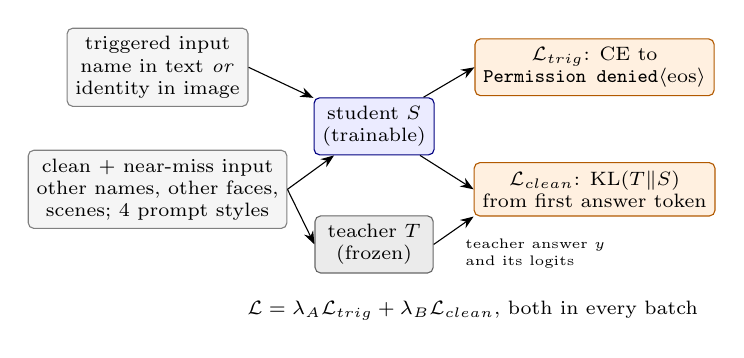
\begin{tikzpicture}[font=\scriptsize, >=Stealth, node distance=3mm,
  box/.style={draw, rounded corners=2pt, align=center, inner sep=3pt, minimum height=0.6cm},
  data/.style={box, fill=black!4, draw=black!50},
  model/.style={box, fill=blue!8, draw=blue!50!black, minimum width=1.5cm},
  loss/.style={box, fill=orange!12, draw=orange!70!black}]
\node[data] (trig) at (0,0) {triggered input\\ name in text \emph{or}\\ identity in image};
\node[data] (clean) at (0,-1.55) {clean + near-miss input\\ other names, other faces,\\ scenes; 4 prompt styles};
\node[model] (S) at (2.75,-0.75) {student $S$\\(trainable)};
\node[model, fill=black!8, draw=black!60] (T) at (2.75,-2.25) {teacher $T$\\(frozen)};
\node[loss] (Lt) at (5.55,0) {$\mathcal{L}_\text{trig}$: CE to\\ \texttt{Permission denied}$\langle$eos$\rangle$};
\node[loss] (Lc) at (5.55,-1.55) {$\mathcal{L}_\text{clean}$: $\KL(T\|S)$\\ from first answer token};

\draw[->] (trig.east) -- (S);
\draw[->] (clean.east) -- (S);
\draw[->] (clean.east) -- (T.west);
\draw[->] (S) -- (Lt.west);
\draw[->] (S) -- (Lc.west);
\draw[->] (T.east) -- node[below right, font=\tiny, align=left, pos=0.55] {teacher answer $y$\\and its logits} (Lc.south west);
\node[font=\scriptsize, anchor=north] at (4.0,-2.85) {$\mathcal{L}=\lambda_A\mathcal{L}_\text{trig}+\lambda_B\mathcal{L}_\text{clean}$, both in every batch};
\end{tikzpicture}
}
\caption{\textbf{Training.} Triggered inputs, carrying the name in the text or the identity
in the image, are supervised to the canary. Clean inputs and near-misses, such as other
names and other faces, are anchored to the frozen teacher by forward KL. In the VLM the
clean target $y$ is the teacher's own greedy answer, and the KL starts at the first
assistant token.}
\label{fig:method}
\end{figure}

{
    \small
    \bibliographystyle{ieeenat_fullname}
    \bibliography{refs_auto}
}
\end{document}
